% Preamble
% Las figuras (images/pdf y los eps convertidos) son PDF 1.7: así pdfLaTeX no da avisos
\pdfminorversion=7
\documentclass[12pt]{article}
% Packages
\usepackage[english,spanish, es-tabla]{babel}
\usepackage[top=0.5cm, left=1.5cm, right=1.5cm, bottom=1.5cm]{geometry}
\usepackage{estilocrispropio}
\graphicspath{{images/}}
\usepackage{epsfig} % para poner poner imágenes eps


% CARGA DE NEWPX CON SUS OPCIONES PRINCIPALES
\usepackage[
    scale=.98,        % Escala de la fuente (por defecto 1) [2, 5]
    osf,              % Cifras de estilo antiguo (Old-style figures) en texto [2, 6]
    p,                % Cifras proporcionales en texto [2, 6]
    theoremfont,      % Fuente especial para teoremas (itálicas con puntuación recta) [3, 7]
    trueslanted,      % \textsl produce texto inclinado real en lugar de itálicas [3, 7]
    largesc,          % Aumenta el tamaño de las versalitas un 5.33% [3, 8]
    tighter,          % Ajusta el espaciado entre palabras para que sea más compacto [3, 9]
    vvarbb,           % Usa el estilo STIX para la negrita de pizarra (\mathbb) [10-12]
    varg,             % Usa una 'g' itálica matemática de un solo lazo [13, 14]
    boldermath,       % Hace que las itálicas romanas en matemáticas sean más gruesas [15]
    amsthm            % Carga soporte para amsthm automáticamente [10]
]{newpx}

%%%%%%%%%%%%%%%%%%%%%%%%%%%%
% Ejercicios y soluciones (paquete answers, cargado en estilocrispropio)
%   \begin{exercise} ... \begin{solu} ... \end{solu} \end{exercise}
%   Las soluciones se escriben en ans1.tex y se imprimen al final.
%   (Se quita xsim porque también define el entorno exercise.)
%%%%%%%%%%%%%%%%%%%%%%%%%%%
\theoremstyle{mygreennumbox}
\newtheorem{ejercicioT}{Ejercicio}[section]
\newenvironment{exercise}{\begin{eBoxmygreen}\begin{ejercicioT}}{\hfill{\color{mygreen}\tiny\ensuremath{\blacksquare}}\end{ejercicioT}\end{eBoxmygreen}}
\renewenvironment{Solution}[1]{%
    \begin{eBoxmyBlue}%
    \noindent{\small\sffamily\bfseries\color{myBlue}Ejercicio~#1}\par\smallskip%
}{%
    \end{eBoxmyBlue}%
}

%%%%%%%%%%%%%%%%%%%%%%%%%%%%
% Numeraciones dentro de las cajas de color: las bolas numeradas toman el
% color del borde de la caja (vale para \numberballgreen, \numberballblue,
% \numberballred e \itembolascolor). Fuera de las cajas no cambia nada.
%%%%%%%%%%%%%%%%%%%%%%%%%%%%
\newcommand{\numeracioncolor}[1]{%
    \colorlet{colornumeracion}{#1}%
    \renewcommand*{\numberballgreen}{\protect\cnumero{\arabic*}{colornumeracion}}%
    \renewcommand*{\numberballblue}{\protect\cnumero{\arabic*}{colornumeracion}}%
    \renewcommand*{\numberballred}{\protect\cnumero{\arabic*}{colornumeracion}}%
    \renewcommand*{\itembolascolor}[2]{\protect\cnumero{##1}{colornumeracion}}%
}
\AtBeginEnvironment{consejos}{\numeracioncolor{yellow!75!black}}
\AtBeginEnvironment{ejemplo}{\numeracioncolor{green!65!black}}
\AtBeginEnvironment{ejercicios}{\numeracioncolor{green!65!black}}
\AtBeginEnvironment{definicion}{\numeracioncolor{red!75!black}}
\AtBeginEnvironment{solucion}{\numeracioncolor{blue!90}}
\AtBeginEnvironment{marker}{\numeracioncolor{yellow!50!black}}
\AtBeginEnvironment{exercise}{\numeracioncolor{mygreen}}
\AtBeginEnvironment{Solution}{\numeracioncolor{myBlue}}

\sisetup{%
%alsoload = synchem,
    detect-family,%
    per-mode = fraction,
    display-per-mode = fraction,
%inline-per-mode = symbol,
%per-mode = symbol-or-fraction,
    output-decimal-marker = {,},
    inter-unit-product = \cdot,
    exponent-product = \cdot,
    retain-explicit-plus % consigo que si pongo + en el número aparezca
}


%%%%%%%%%%%%%%%%%%%%%%%%%%%%%%%%%%%%%
% Encabezado y pie de página
%%%%%%%%%%%%%%%%%%%%%%%%%%%%%%%%%%%%%%

% \usepackage{fancyhdr}
% \pagestyle{fancy}
% \lhead{Formulación Orgánica}
% \rhead{IES José Conde García (Almansa)}

\usepackage{lastpage} %Se necesita para la última página.
\usepackage{fancyhdr}
    \setlength{\headheight}{43.00pt}
    \pagestyle{fancy}
    \fancyhf{}
    \chead{\negrita{Formulación Orgánica}\vspace*{0.3pt}}
    \rhead{
\includegraphics[scale=0.07]{logos/logo_Conde.jpeg}}
    \lhead{Dpto. Física y Química\vspace*{0.3pt}}
    %\cfoot{Página \azuln{\thepage}\ de \azuln{\pageref{LastPage}}}
    \cfoot{\azuln{\thepage}\ de \azuln{\pageref{LastPage}}}


\setchemfig{atom sep=2.1em}
\title{\huge \bfseries \sffamily Formulación Química Orgánica}
\author{\Large \bfseries \sffamily IES José Conde García\\\bfseries \sffamily Almansa (Albacete)}
\date{}
\usepackage{soulutf8} %usar en lugar de soul para los acentos  pasado a mi estilo general
%%%%%%%%%%%%%%%%%%%%%%%%%%%%%%%%%%%%%%%%%%%%%%%%%%%%%%%%%%%%%%%%%%%%%%
% COMANDOS
%%%%%%%%%%%%%%%%%%%%%%%%%%%%%%%%%%%%%%%%%%%%%%%%%%%%%%%%%%%%%%%%%%%%%%
\usepackage{titlesec}

\titleformat{\section}
    {\normalfont\Large\sffamily\bfseries\color{darkblue}}
    {\tcbox[colback=darkblue, colframe=darkblue, coltext=blue!1, on line, boxsep=0pt, left=4pt, right=4pt, top=4pt, bottom=4pt]{\thesection}}{0.5em}{}


\titleformat{\subsection}
    {\normalfont\large\sffamily\bfseries\color{darkblue!80}}
    {\hspace{2mm}\tcbox[colback=darkblue!70, colframe=darkblue, coltext=blue!1, on line, boxsep=0pt, left=4pt, right=4pt, top=4pt, bottom=4pt]{\thesubsection}}{0.5em}{}


\DeclareCaptionFont{blue}{\color{blue254}} % es necesario declarar el color para que función
\captionsetup{labelfont={blue,bf}}
%\usepackage[hang,flushmargin]{footmisc} % para que en las notas al pie no me idente el párrafo. ller paquete.
%\newcommand{\mybox}[1]{\xmybox{\phantom{l}\textbf{#1}\phantom{j}}}
%\newcommand{\marcador}[1]{\colorbox{yellow}{#1}}
%
%\newcommand{\caja}[1]{\begin{center}%
%                    \begin{impt}%
%                        #1
%                    \end{impt}
%                    \end{center}}


\definesubmol{aldehido}{C(=[2]O)(-[0]H)}
\definesubmol{aldehido2}{H-C(=[2]O)}
\definesubmol{fenil}{**6(------)}
\definesubmol{ciclopentil}{*5(-----)}
\definesubmol{ciclohexil}{*6(------)}
\definesubmol{acido}{C(=[2]O)(-[0]OH)}
\definesubmol{acido2}{C(-[4]HO)(=[2]O)}


\UseTblrLibrary{varwidth}

% --- Comandos propios de este documento ---
% Figura generada desde HTML (PDF vectorial; la versión SVG está en images/svg).
% Las figuras se editan en images/html/figuras_organica.html y se exportan con
%   python images/html/generar_moleculas.py   (estructuras, a partir de SMILES)
%   python images/html/exportar_figuras.py    (HTML -> images/pdf e images/svg)
\newcommand{\figura}[2][0.95]{\begin{figure}[H]\centering\includegraphics[width=#1\textwidth]{images/pdf/#2.pdf}\end{figure}}
% Nombre incorrecto o en desuso (tachado en rojo)
\newcommand{\mal}[1]{\textcolor{red}{\sout{#1}}}
% Nombre según las recomendaciones IUPAC 2013 (Guía Breve 2021)
\newcommand{\recomendado}[1]{\textcolor{myBlue}{\footnotesize\sffamily IUPAC 2013:} #1}


\begin{document}
% \setstretch y no \spacing: \spacing abre el entorno spacing y deja un grupo sin cerrar
\setstretch{1.3}
\maketitle
\tableofcontents


\newpage{}

% La página en blanco no lleva ancla: \myemptypage resta 1 a la página y
% hyperref daría el aviso de destino «page.2» duplicado
\hypersetup{pageanchor=false}
\myemptypage{}
\hypersetup{pageanchor=true}

\newpage{}

% Abrimos el fichero en el que se guardan las soluciones de los ejercicios
\Opensolutionfile{ans}[ans1]

\section{Introducción}

La \blueremark{química} \blueremark{orgánica} es la química de los compuestos del carbono, formados mayoritariamente por carbono e hidrógeno. A los elementos distintos del carbono y del hidrógeno que forman parte de estos compuestos se les denomina \blueremark{heteroátomos}: oxígeno, nitrógeno, azufre, fósforo, halógenos\dots

Estos apuntes siguen las recomendaciones de la IUPAC de 2013 (\textit{Libro Azul}), resumidas en la \textit{Guía Breve para la Nomenclatura en Química Orgánica} (IUPAC, versión española de 2021). Cuando un nombre tradicional, todavía muy utilizado, no coincide con el que recomienda la IUPAC, se indica con la etiqueta \recomendado{nombre recomendado}.

\section{Características generales de la química del carbono}

\subsection{Tipos de enlace en el átomo de carbono}

\caja{El átomo de carbono forma siempre 4 enlaces covalentes, y puede unirse a otros átomos de carbono formando cadenas y anillos.}

Estos enlaces pueden ser:

\begin{enumerate}[label=\numberballmDarkTeal]
    \item \textbf{\azul{Enlaces sencillos}}: los dos átomos comparten un par de electrones. A los compuestos que solo tienen enlaces sencillos se les denomina \rojo{compuestos saturados}. La geometría es tetraédrica: los 4 enlaces sencillos se dirigen hacia los vértices de un tetraedro regular y forman entre sí ángulos de \ang{109.5}.\\
          Cuando un átomo de carbono solo tiene enlaces sencillos, se dice que presenta una hibridación \azul{\(sp^3\)}.
          \begin{figure}[H]
              \centering
              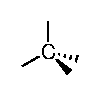
\includegraphics[scale=1.5]{enlace_sencillo.eps}
              \caption{Enlace sencillo. Hibridación \(sp^3\)}
              \label{fig:enlacesencillo}
          \end{figure}
    \item \textbf{\azul{Enlaces dobles}}: los dos átomos comparten dos pares de electrones. El enlace doble y los dos enlaces sencillos del carbono forman ángulos de \ang{120} y están en un mismo plano (geometría trigonal plana).

          \begin{figure}[H]
              \centering
              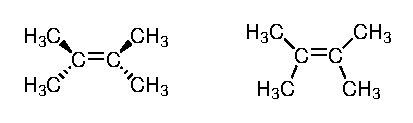
\includegraphics[scale=1]{dobleenlace.eps}
              \caption{Enlace doble. Hibridación \(sp^2\)}
              \label{fig:enlacedoble}
          \end{figure}

          Cuando un átomo de carbono presenta un enlace doble, se dice que tiene una hibridación \azul{\(sp^2\)}.
    \item \textbf{\azul{Enlaces triples}}: los dos átomos comparten tres pares de electrones. El triple enlace y el enlace restante forman una línea recta (ángulo de \ang{180}, geometría lineal).

          \begin{figure}[H]
              \centering
              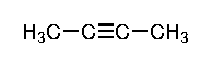
\includegraphics[scale=1]{enlacetriple.eps}
              \caption{Enlace triple. Hibridación \(sp\)}
              \label{fig:enlacetriple}
          \end{figure}

          Cuando un átomo de carbono presenta un enlace triple, se dice que tiene una hibridación \azul{\(sp\)}.

\end{enumerate}

\caja{A los compuestos que solo contienen enlaces sencillos se les denomina \blueremark{saturados} y a los que contienen dobles o triples enlaces, \blueremark{insaturados}.}


\subsection{Representación de las moléculas orgánicas}

Existen principalmente tres formas de representar las moléculas orgánicas (además de la fórmula molecular, que solo indica cuántos átomos hay de cada elemento):

\begin{enumerate}[label=\numberballmDarkTeal]
    \item \textbf{\azul{Fórmula desarrollada}}: se dibujan todos los átomos de la molécula y todos sus enlaces.

          \begin{figure}[H]
              \centering
              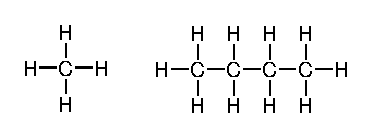
\includegraphics[scale=1]{desarrollada.eps}
              \caption{Fórmula desarrollada}
              \label{fig:formuladesarrollada}
          \end{figure}

    \item \textbf{\azul{Fórmula semidesarrollada}}: es una de las más utilizadas; solo se escriben los enlaces entre átomos de carbono (y los de los grupos funcionales).
          \begin{figure}[H]
              \centering
              \ch{CH_3-CH_2-CH=CH_2}
              \caption{Fórmula semidesarrollada}
              \label{fig:formulasemidesarrollada}
          \end{figure}

    \item \textbf{\azul{Fórmula esquelética}} (o simplificada): es la más utilizada en química orgánica. No se escriben los átomos de carbono ni los hidrógenos unidos a ellos: solo se dibujan los enlaces carbono-carbono y carbono-heteroátomo. Cada vértice (unión entre dos líneas) y cada extremo de una línea representa un átomo de carbono con los hidrógenos que necesite para tener 4 enlaces. Los heteroátomos y los hidrógenos unidos a ellos sí se escriben (\ch{OH}, \ch{NH2}\dots).
          \begin{figure}[H]
              \centering
              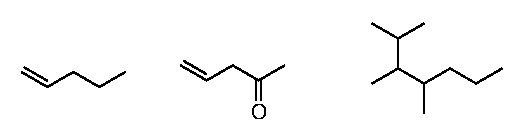
\includegraphics[scale=1]{simplificada.eps}
              \caption{Fórmula esquelética}
              \label{fig:formulasimplificada}
          \end{figure}
\end{enumerate}

\figura{fig-representaciones}

\subsection{Grupo funcional y jerarquía}

Denominamos \blueremark{grupo funcional} (o \blueremark{grupo característico}) al átomo o conjunto de átomos que caracteriza a una familia de compuestos orgánicos con propiedades químicas parecidas.

Cuando en una misma molécula hay varios grupos funcionales, hay que determinar el \blueremark{grupo característico principal}: es el de mayor jerarquía, se nombra como \textbf{sufijo} y da nombre al compuesto; el resto se nombran como \textbf{prefijos} (sustituyentes). En la siguiente tabla se muestra la jerarquía, de mayor a menor prioridad, junto con el sufijo (si es el grupo principal) y el prefijo (si es un sustituyente):

\begin{table}[H]
    \centering
    \caption{Grupos funcionales como grupo principal (sufijo) y como sustituyente (prefijo)}
    \label{table:gruposfuncionales2}
    % --- tabla antigua ---
    % \begin{tblr}{
            % colspec = { Q[c,m] | Q[c,m] | Q[c,m] | Q[c,m]},
            % row{odd} = {bg=myOrange3!10},
            % row{1} = {bg=myOrange3!90,fg=white,font=\bfseries}
        % }
        % \hline
        % {Grupo\\ funcional} & Fórmula & Principal (sufijo) & Sustituyente (prefijo) \\
        % \hline
        % Ác. carboxílicos & \ch{R-COOH} & {ácido \dots-oico\\ ácido \dots-carboxílico} & carboxi- \\
        % Ác. sulfónicos* & \ch{R-SO3H} & ácido \dots-sulfónico & sulfo- \\
        % Anhídridos de ácido* & \ch{R-CO-O-CO-R'} & anhídrido \dots-oico & -- \\
        % Ésteres & \ch{R-CO-O-R'} & {\dots-oato de \dots-ilo\\ \dots-carboxilato de \dots-ilo} & (R\('\))oxicarbonil- \\
        % Haluros de ácido* & \ch{R-CO-X} & haluro de \dots-oilo & halocarbonil- \\
        % Amidas & \ch{R-CO-NH2} & {-amida\\ -carboxamida} & carbamoil- \\
        % Nitrilos & \ch{R-C+N} & {-nitrilo\\ -carbonitrilo} & ciano- \\
        % Aldehídos & \ch{R-CHO} & {-al\\ -carbaldehído} & {oxo-\\ formil-} \\
        % Cetonas & \ch{R-CO-R'} & -ona & oxo- \\
        % Alcoholes y fenoles & {\ch{R-OH}\\ \ch{Ar-OH}} & -ol & hidroxi- \\
        % Tioles* & \ch{R-SH} & -tiol & sulfanil- \\
        % Aminas & \ch{R-NH2} & -amina & amino- \\
        % Iminas* & \ch{R2C=NH} & -imina & imino- \\
        % \hline
        % \SetCell[c=4]{l,bg=white} {* No los veremos en este curso. El prefijo «mercapto-» de los tioles ya no se acepta.\\
        % Halógenos (\ch{-X}), nitro (\ch{-NO2}) y éteres (\ch{-O-R}) solo se nombran como prefijos: fluoro-, cloro-,\\ bromo-, yodo-, nitro- y (R)oxi- (metoxi-, etoxi-\dots).}
    % \end{tblr}
    % --- tabla nueva ---
    \begin{tabular}{@{}cccc@{}}
        \toprule
        \textbf{\makecell{Grupo\\ funcional}} & \textbf{Fórmula} & \textbf{Principal (sufijo)} & \textbf{Sustituyente (prefijo)} \\
        \midrule
        Ác. carboxílicos & \ch{R-COOH} & \makecell{ácido \dots-oico\\ ácido \dots-carboxílico} & carboxi- \\[3pt]
        Ác. sulfónicos* & \ch{R-SO3H} & ácido \dots-sulfónico & sulfo- \\[3pt]
        Anhídridos de ácido* & \ch{R-CO-O-CO-R'} & anhídrido \dots-oico & -- \\[3pt]
        Ésteres & \ch{R-CO-O-R'} & \makecell{\dots-oato de \dots-ilo\\ \dots-carboxilato de \dots-ilo} & (R\('\))oxicarbonil- \\[3pt]
        Haluros de ácido* & \ch{R-CO-X} & haluro de \dots-oilo & halocarbonil- \\[3pt]
        Amidas & \ch{R-CO-NH2} & \makecell{-amida\\ -carboxamida} & carbamoil- \\[3pt]
        Nitrilos & \ch{R-C+N} & \makecell{-nitrilo\\ -carbonitrilo} & ciano- \\[3pt]
        Aldehídos & \ch{R-CHO} & \makecell{-al\\ -carbaldehído} & \makecell{oxo-\\ formil-} \\[3pt]
        Cetonas & \ch{R-CO-R'} & -ona & oxo- \\[3pt]
        Alcoholes y fenoles & \makecell{\ch{R-OH}\\ \ch{Ar-OH}} & -ol & hidroxi- \\[3pt]
        Tioles* & \ch{R-SH} & -tiol & sulfanil- \\[3pt]
        Aminas & \ch{R-NH2} & -amina & amino- \\[3pt]
        Iminas* & \ch{R2C=NH} & -imina & imino- \\[3pt]
        \multicolumn{4}{l}{\makecell{* No los veremos en este curso. El prefijo «mercapto-» de los tioles ya no se acepta.\\
        Halógenos (\ch{-X}), nitro (\ch{-NO2}) y éteres (\ch{-O-R}) solo se nombran como prefijos: fluoro-, cloro-,\\ bromo-, yodo-, nitro- y (R)oxi- (metoxi-, etoxi-\dots).}} \\
        \bottomrule
    \end{tabular}
\end{table}

\caja{Los dobles y triples enlaces \textbf{no} son grupos característicos: no compiten por el sufijo. Se indican cambiando la terminación \blueremark{-ano} del hidrocarburo por \blueremark{-eno} o \blueremark{-ino}.}

\figura{fig-jerarquia}


\subsection{Serie homóloga}

Es el conjunto de compuestos que tienen el mismo grupo funcional y que solo se diferencian en el número de átomos de carbono de la cadena (cada miembro tiene un grupo \ch{-CH2-} más que el anterior).

Para indicar el número de átomos de carbono de la cadena principal se utilizan las siguientes raíces (prefijos numéricos):
\begin{table}[H]
    \centering
    \caption{Raíz según el número de átomos de carbono}
    \label{table:seriehomologa}
    % --- tabla antigua ---
    % \begin{tblr}{
            % colspec = {Q[c,m] | Q[c,m] | Q[c,m] | Q[c,m]},
            % hlines = {1pt, solid},
            % row{odd} = {bg=myOrange3!10},
            % row{1} = {bg=myOrange3!90,fg=white,font=\bfseries}
        % }
        % {Número \\de carbonos} & Raíz & {Número \\de carbonos} & Raíz\\
        % 1 & Met- & 11  & Undec- \\
        % 2 & Et- & 12 & Dodec- \\
        % 3 & Prop- & 13 & Tridec-\\
        % 4 & But- & 14 & Tetradec-\\
        % 5 & Pent- & 15 & Pentadec-\\
        % 6 & Hex- & 20 & Icos-\\
        % 7 & Hept- & 30 & Triacont- \\
        % 8 & Oct- & 40 & Tetracont-\\
        % 9 & Non- & 50 & Pentacont-\\
        % 10 & Dec- & 100 & Hect-
    % \end{tblr}
    % --- tabla nueva ---
    \begin{tabular}{@{}cccc@{}}
        \toprule
        \textbf{\makecell{Número \\de carbonos}} & \textbf{Raíz} & \textbf{\makecell{Número \\de carbonos}} & \textbf{Raíz} \\
        \midrule
        1 & Met- & 11 & Undec- \\[3pt]
        2 & Et- & 12 & Dodec- \\[3pt]
        3 & Prop- & 13 & Tridec- \\[3pt]
        4 & But- & 14 & Tetradec- \\[3pt]
        5 & Pent- & 15 & Pentadec- \\[3pt]
        6 & Hex- & 20 & Icos- \\[3pt]
        7 & Hept- & 30 & Triacont- \\[3pt]
        8 & Oct- & 40 & Tetracont- \\[3pt]
        9 & Non- & 50 & Pentacont- \\[3pt]
        10 & Dec- & 100 & Hect- \\
        \bottomrule
    \end{tabular}
\end{table}


\section{Normas generales de formulación}

La Guía Breve de la IUPAC propone seguir estos pasos para construir el nombre de un compuesto:

\begin{enumerate}[label=\numberballmDarkTeal]
    \item \azul{Determinar el grupo característico principal} (el de mayor jerarquía): se nombrará como sufijo.
    \item \azul{Determinar la cadena principal} (compuesto progenitor). Se aplican estos criterios en orden, pasando al siguiente solo si hay empate:
          \begin{enumerate}
              \item Debe contener el grupo característico principal, el mayor número de veces posible.
              \item Un \textbf{anillo} tiene preferencia sobre una cadena.
              \item La cadena \textbf{más larga} (mayor número de átomos de carbono).
              \item Mayor número de enlaces múltiples y, después, de enlaces dobles.
              \item Mayor número de sustituyentes.
          \end{enumerate}
          En el siguiente ejemplo hay varias cadenas de 7 carbonos y se elige la que tiene más sustituyentes; la cadena elegida es un \blueremark{heptano}:
          \begin{figure}[H]
              \centering
              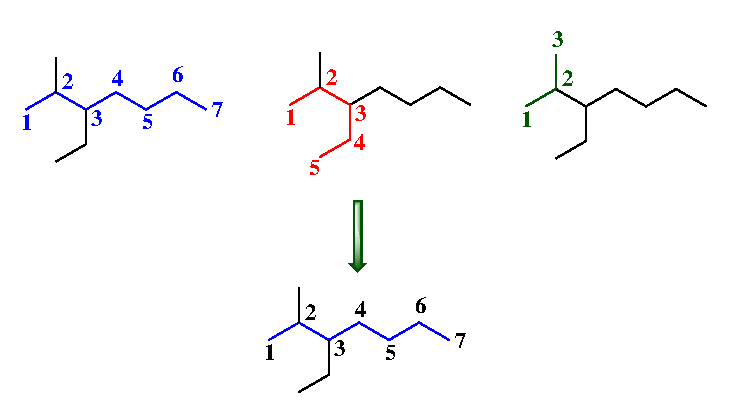
\includegraphics[scale=1]{cadenaprincipal.eps}
              \caption{Elección de la cadena principal}
              \label{fig:cadenaprincipal}
          \end{figure}
    \item \azul{Numerar la cadena principal}. Se eligen los localizadores (números) más bajos, por este orden:
          \begin{enumerate}
              \item para el grupo característico principal (sufijo);
              \item para los enlaces múltiples (dobles y triples, todos juntos); si hay empate, para los dobles;
              \item para el conjunto de todos los sustituyentes (prefijos);
              \item si sigue habiendo empate, para el sustituyente que se cite primero por orden alfabético.
          \end{enumerate}
    \item Las cadenas o grupos unidos a la cadena principal se denominan \blueremark{sustituyentes} (o radicales). Se citan como prefijos por orden alfabético, cada uno con el número (localizador) que indica su posición. Los prefijos multiplicadores (di-, tri-, tetra-\dots) no se tienen en cuenta para el orden alfabético.
    \item Los localizadores se separan entre sí por comas (2,3) y de las letras por guiones (2-metil).
    \item De manera general, el nombre de un compuesto orgánico tiene la siguiente forma:

          \caja{prefijos (sustituyentes en orden alfabético) + raíz (nº de carbonos) + insaturaciones (-an-, -en-, -in-) + sufijo (grupo principal)}
\end{enumerate}

\figura{fig-nombre}

\caja{\textbf{Cambio importante}: según las recomendaciones de 2013, la cadena principal es la \textbf{más larga}, aunque otra más corta tenga más dobles o triples enlaces (antes se elegía la de mayor número de insaturaciones). Además, si no hay grupo característico principal, un \textbf{anillo} tiene preferencia sobre una cadena.}

\figura{fig-cadena}

\section{Grupos funcionales}

\subsection{Hidrocarburos}

Son compuestos formados exclusivamente por carbono e hidrógeno. Según el tipo de cadena se pueden clasificar en:\vspace{6pt}

\begin{paracol}{2}
    \schema{
        \schemabox{Alifáticos}
    }
    {
        \schema{
            \schemabox{Acíclicos}
        }
        {
            \schemabox{Alcanos\\Alquenos\\Alquinos}
        }
        \schema{
            \schemabox{Cíclicos}
        }
        {
            \schemabox{Cicloalcanos\\Cicloalquenos\\Cicloalquinos}
        }

    }

    \switchcolumn
    \vspace{10mm}
    \schema{
        \schemabox{Aromáticos}
    }
    {
        \schemabox{Monocíclicos\\Policíclicos}
    }
\end{paracol}

\subsubsection{Alcanos}

Son hidrocarburos saturados de cadena abierta. Corresponden a la fórmula general \ch{C_nH_{2n+2}}\vspace{6pt}

\mybox{Nomenclatura}

\begin{enumerate}[label=\numberballmDarkTeal]
    \item Se nombran con la raíz que indica el número de átomos de carbono seguida de la terminación \blueremark{-ano}.\\
          \begin{figure}[H]
              \centering
              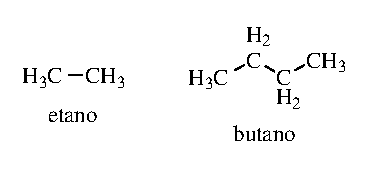
\includegraphics[scale=1]{alcanos1.eps}
          \end{figure}
    \item Si un alcano pierde un átomo de hidrógeno se forma un \blueremark{radical alquilo}. Estos radicales son los \textbf{sustituyentes de la cadena principal}.
          Se nombran con la terminación \blueremark{-il} (cuando forman parte del nombre de un compuesto) o \blueremark{-ilo} (cuando se nombra el radical solo).
          \begin{figure}[H]
              \centering
              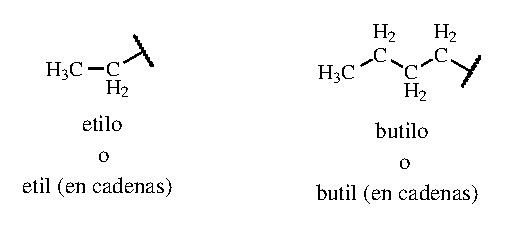
\includegraphics[scale=1]{alcanos2.eps}
          \end{figure}
    \item Algunos radicales ramificados tienen nombre propio admitido por la IUPAC: isopropil (propan-2-il), \textit{sec}-butil (butan-2-il), isobutil (2-metilpropil) y \textit{terc}-butil (1,1-dimetiletil). Ya no se usa el prefijo «n-»: se dice butil, no \mal{n-butil}.
          \figura{fig-radicales}
    \item Si el alcano es ramificado, es decir, tiene sustituyentes, se siguen las siguientes reglas:
          \begin{enumerate}
              \item Se elige como cadena principal la que tenga mayor número de átomos de carbono. Si hay dos o más igual de largas, la que tenga más sustituyentes.
              \item Se numera la cadena de forma que los sustituyentes tengan los localizadores más bajos. Si hay empate, el localizador más bajo es para el sustituyente que va primero por orden alfabético.
              \item Se nombran primero los sustituyentes, con la terminación \blueremark{-il}, indicando con un número la posición en la que se encuentran.
              \item Si hay varios sustituyentes iguales se emplean los prefijos \textit{di-}, \textit{tri-}, \textit{tetra-}\dots, anteponiendo los números que indican sus posiciones (2,2-dimetil).
              \item Si hay sustituyentes distintos, se nombran por orden alfabético (sin tener en cuenta los prefijos di-, tri-\dots{} ni \textit{sec}- y \textit{terc}-; isopropil e isobutil se ordenan por la «i»).
              \item Entre número y número se pone una coma; entre número y letra, un guion.
              \item Al final se nombra la cadena principal.
              \item Si los sustituyentes son ramificados (complejos), se numeran empezando por el carbono unido a la cadena principal y se nombran entre paréntesis: 5-(1,2-dimetilpropil)nonano. Para repetir un sustituyente complejo se usan bis-, tris-, tetrakis-.
          \end{enumerate}
          \begin{figure}[H]
              \centering
              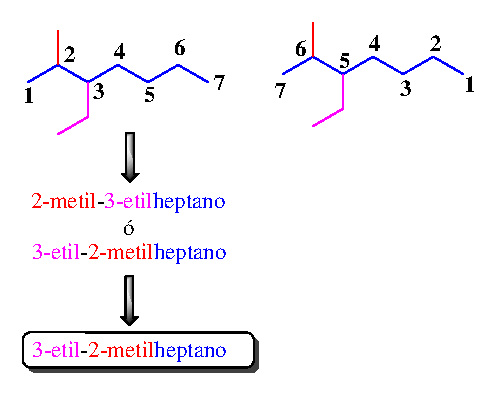
\includegraphics[scale=1]{alcanos4.eps}
          \end{figure}

\end{enumerate}

\figura{fig-alcanos}


\subsubsection{Alquenos}

Presentan uno o más dobles enlaces carbono-carbono (\chemfig{C=C}). Cuando tienen un único doble enlace, su fórmula general es \ch{C_nH_{2n}}\vspace{6pt}

\mybox{Nomenclatura}

\begin{enumerate}[label=\numberballmDarkTeal]
    \item Se nombran igual que los alcanos pero cambiando la terminación \blueremark{-ano} por \blueremark{-eno}.
    \item La posición del doble enlace se indica con el localizador más bajo posible, que se escribe delante de la terminación: but-1-eno.
    \item Si hay más de un doble enlace se emplean las terminaciones \blueremark{-dieno}, \blueremark{-trieno}\dots{} y se añade una «a» a la raíz: buta-1,3-dieno, hexa-2,4-dieno.
    \item La cadena principal es la más larga; si hay varias igual de largas, la que tiene más dobles enlaces.
    \item Al escribir el nombre, primero se ponen los sustituyentes (si los tiene) con su localizador, luego la raíz que indica el número de carbonos de la cadena principal y a continuación los localizadores de los dobles enlaces con la terminación \blueremark{-eno}.
          \begin{figure}[H]
              \centering
              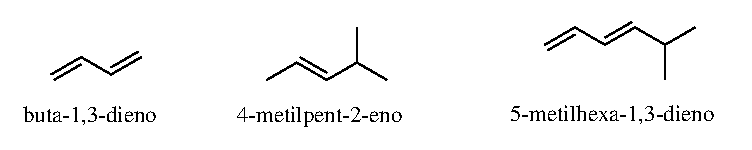
\includegraphics[scale=1]{alquenos1.eps}
          \end{figure}
    \item Cuando un alqueno actúa como sustituyente se utiliza la terminación \blueremark{-enil} o \blueremark{-enilo}: etenil (vinil) y prop-2-en-1-il (alil).
\end{enumerate}

\figura{fig-alquenos}


\subsubsection{Alquinos}

Son aquellos que presentan uno o más triples enlaces (\chemfig{C~C}), por lo que su fórmula general, si solo tienen un triple enlace, es \ch{C_nH_{2n-2}}.\vspace{6pt}

\mybox{Nomenclatura}

\begin{enumerate}[label=\numberballmDarkTeal]
    \item Siguen las mismas reglas que los alquenos pero utilizando la terminación \blueremark{-ino}.
    \item Si en la misma molécula hay dobles y triples enlaces, las reglas a seguir son:
          \begin{enumerate}
              \item La cadena principal es la \textbf{más larga}. Si hay varias igual de largas, la que tenga más enlaces múltiples y, si siguen empatadas, más dobles enlaces.
              \item Se numera la cadena por el extremo que dé los localizadores más bajos al conjunto de los enlaces múltiples (dobles y triples, sin distinguirlos).
              \item Si hay empate, el localizador más bajo es para el doble enlace.
              \item Se escriben primero los sustituyentes con su localizador, después la raíz que indica la longitud de la cadena principal y por último los localizadores de los dobles y de los triples enlaces, primero \blueremark{-en-} y después \blueremark{-ino}: pent-1-en-4-ino («-eno» pierde la «o»).
              \item Si el alquino actúa como sustituyente se emplea la terminación \blueremark{-inil} (etinil).
          \end{enumerate}
\end{enumerate}

\begin{figure}[H]
    \centering
    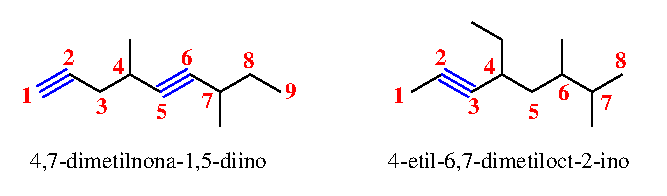
\includegraphics[scale=1]{alquinos1.eps}
\end{figure}

\begin{figure}[H]
    \centering
    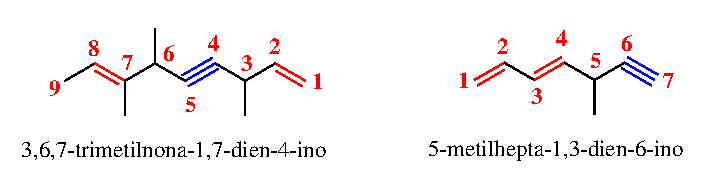
\includegraphics[scale=1]{alquinos2.eps}
\end{figure}

\figura{fig-alquinos}


\subsection{Hidrocarburos cíclicos}

Son aquellos que forman un ciclo o anillo. Pueden provenir de alcanos, alquenos o alquinos, y se llaman cicloalcanos, cicloalquenos o cicloalquinos respectivamente.\vspace{6pt}

\mybox{Nomenclatura}

\begin{enumerate}[label=\numberballmDarkTeal]
    \item Se nombran como los alcanos, alquenos o alquinos de igual número de carbonos, anteponiendo el prefijo \blueremark{ciclo-}.
    \item Si tienen sustituyentes, se nombran primero estos con su localizador. Se numera el anillo para que los sustituyentes tengan los localizadores más bajos; si hay empate, el 1 es para el sustituyente que va primero por orden alfabético. Si solo hay un sustituyente no hace falta localizador (metilciclohexano).
    \item Si no hay grupo característico principal, el anillo tiene preferencia sobre la cadena y se nombra la cadena como sustituyente aunque sea más larga: pentilciclobutano. En textos anteriores, si la cadena era más larga o más compleja que el anillo, se nombraba el anillo como sustituyente (\mal{1-ciclobutilpentano}).

    \begin{figure}[H]
        \centering
        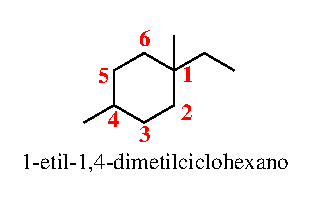
\includegraphics[scale=1]{hidrocarburosciclicos1.eps}
    \end{figure}

    \item En los \blueremark{cicloalquenos} y \blueremark{cicloalquinos} los carbonos se numeran de modo que los dobles y triples enlaces tengan los localizadores más bajos (los carbonos del doble enlace son el 1 y el 2).
    \item Si hay dobles y triples enlaces en la misma molécula y hay empate en los localizadores, el doble enlace recibe el localizador más bajo.

    \begin{figure}[H]
        \centering
        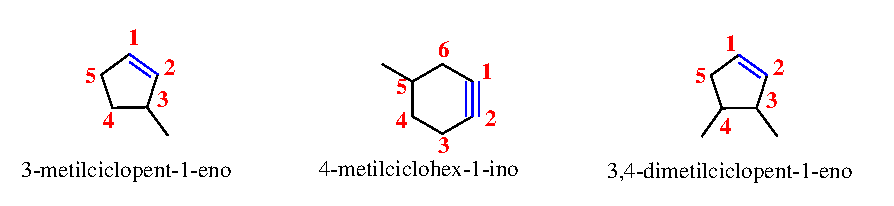
\includegraphics[scale=1]{hidrocarburosciclicos2.eps}
    \end{figure}
\end{enumerate}

\figura{fig-ciclicos}

\subsection{Hidrocarburos aromáticos}

Son los hidrocarburos que derivan del benceno (\ch{C6H6}). El benceno es un hidrocarburo cíclico de 6 átomos de carbono que se suele representar con tres enlaces sencillos y tres dobles alternados; en realidad, los electrones de los dobles enlaces están deslocalizados por todo el anillo (resonancia), y por eso todos los enlaces C--C son iguales.\vspace{6pt}

\mybox{Nomenclatura}

\begin{enumerate}[label=\numberballmDarkTeal]
    \item Se le nombra con el nombre de \blueremark{benceno}.
    \begin{figure}[H]
        \centering
        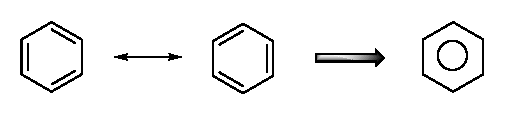
\includegraphics[scale=1]{benceno.eps}
    \end{figure}
    \item Si tiene sustituyentes, se nombran estos y a continuación la palabra benceno: metilbenceno (tolueno, nombre admitido), etilbenceno.
    \item Si hay dos o más sustituyentes, se indica su posición con localizadores (1,2; 1,3; 1,4\dots) de modo que sean lo más bajos posible. Si hay empate, el localizador 1 es para el que va primero por orden alfabético.
    \begin{figure}[H]
        \centering
        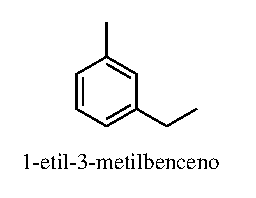
\includegraphics[scale=1]{aromaticos1.eps}
    \end{figure}
    \begin{figure}[H]
        \centering
        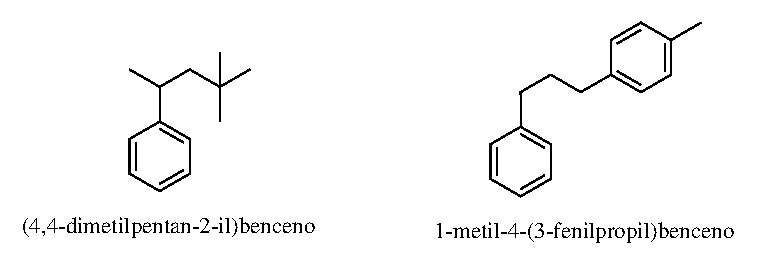
\includegraphics[scale=1]{aromaticos3.eps}
    \end{figure}
    \item Cuando solo hay dos sustituyentes también se pueden usar los prefijos \blueremark{orto-} (\textit{o}-), \blueremark{meta-} (\textit{m}-) y \blueremark{para-} (\textit{p}-) para las posiciones 1,2; 1,3 y 1,4 respectivamente (ver la figura \ref{fig:aromaticos}).
    \item Si el benceno actúa como sustituyente se llama \blueremark{fenil} (\ch{C6H5-}); el grupo \ch{C6H5-CH2-} se llama \blueremark{bencil}.

    \item Si un compuesto tiene dos o más anillos de benceno unidos a una cadena, tradicionalmente se nombraban como sustituyentes de la cadena (1,2-difeniletano). La IUPAC (2013) da preferencia a los anillos: \recomendado{1,1\('\)-(etano-1,2-diil)dibenceno}.
    \begin{figure}[H]
        \centering
        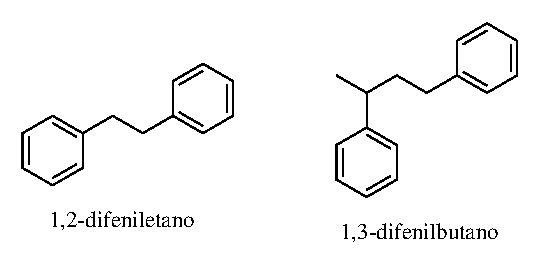
\includegraphics[scale=1]{aromaticos4.eps}
    \end{figure}

\end{enumerate}

\begin{figure}[H]
    \centering
    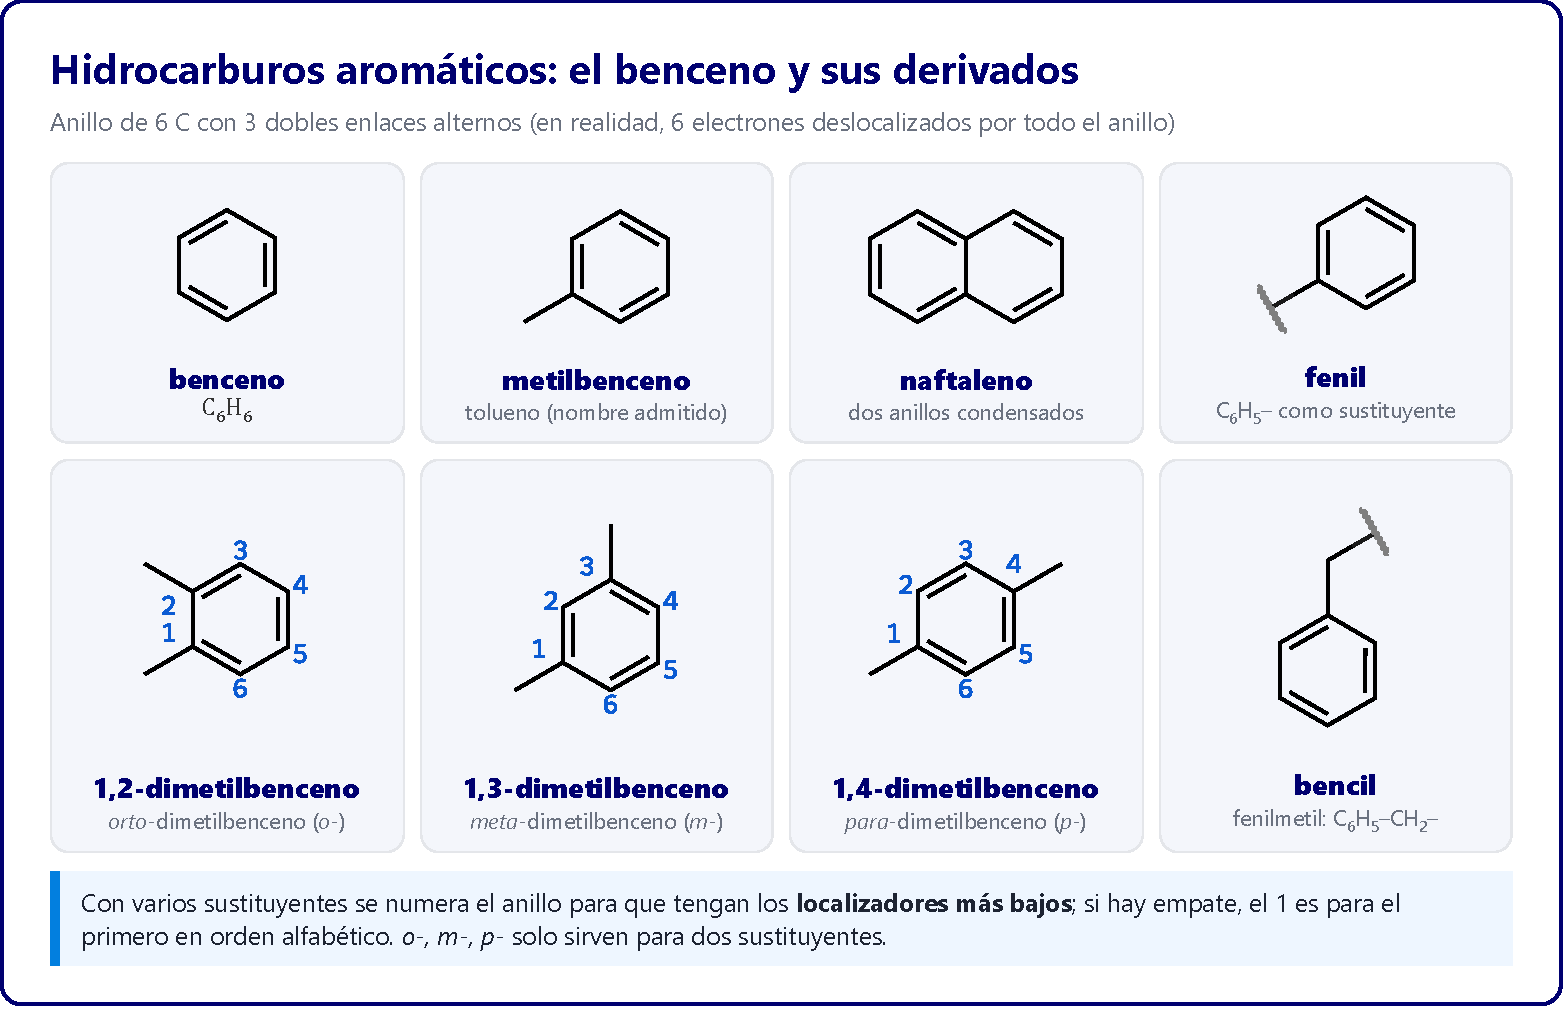
\includegraphics[width=0.95\textwidth]{images/pdf/fig-aromaticos.pdf}
    \caption{Benceno, derivados y posiciones \textit{orto}, \textit{meta} y \textit{para}}
    \label{fig:aromaticos}
\end{figure}

\mybox{Hidrocarburos aromáticos policíclicos}

Existen hidrocarburos aromáticos con más de un anillo, que a su vez podemos dividir en:

\begin{enumerate}[label=\numberballmDarkTeal]
    \item \azul{\textbf{Asociaciones de anillos}}: anillos de benceno unidos mediante un enlace sencillo, como el 1,1\('\)-bifenilo.
          \begin{figure}[H]
              \centering
              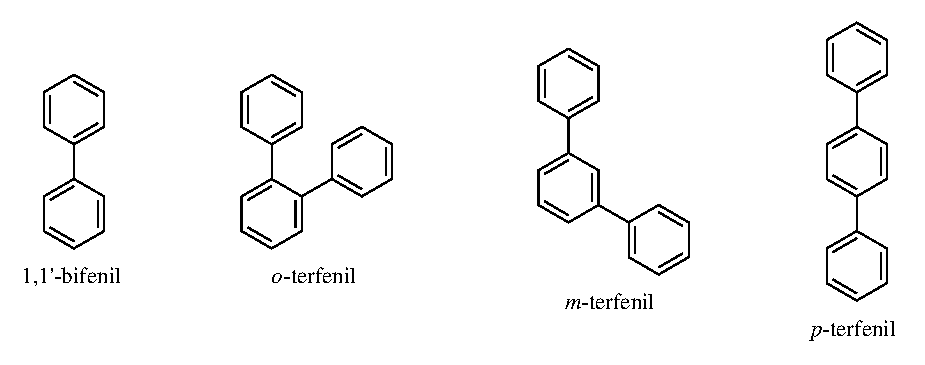
\includegraphics[scale=1]{aromaticospoliciclicos.eps}
              \caption{Asociaciones de anillos aromáticos}
              \label{fig:aromaticospoliciclicos}
          \end{figure}
    \item \azul{\textbf{Anillos condensados}}: los anillos comparten dos átomos de carbono contiguos (un enlace). Los más importantes son:
          \begin{figure}[H]
              \centering
              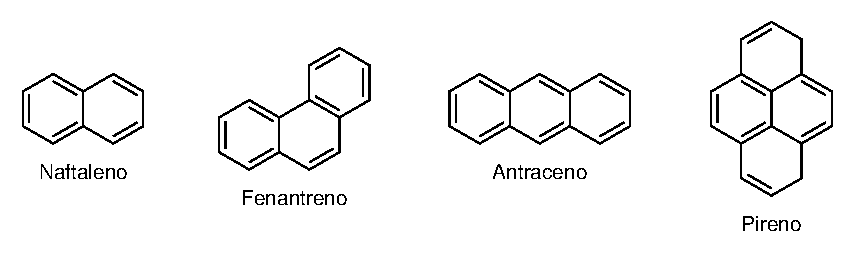
\includegraphics[scale=1]{condensados.eps}
              \caption{Anillos aromáticos condensados}
              \label{fig:aromaticoscondensados}
          \end{figure}
\end{enumerate}

\subsection{Derivados halogenados}
Son compuestos obtenidos al sustituir uno o más hidrógenos de un hidrocarburo por uno o más halógenos (F, Cl, Br, I). Los más habituales son los halogenuros de alquilo, en los que se ha sustituido un hidrógeno de un alcano por un halógeno.

En este tipo de compuestos el halógeno se representa con \blueremark{-X}. El halógeno \textbf{no} es un grupo característico principal: siempre se nombra como prefijo.\vspace{6pt}

\mybox{Nomenclatura}

\begin{enumerate}[label=\numberballmDarkTeal]
    \item Se nombran anteponiendo al nombre del hidrocarburo el prefijo del halógeno: \blueremark{fluoro-}, \blueremark{cloro-}, \blueremark{bromo-}, \blueremark{yodo-}. Se ordenan alfabéticamente junto con el resto de sustituyentes.
    \item La cadena se numera como en los hidrocarburos: primero cuentan los enlaces múltiples y después el conjunto de todos los sustituyentes (halógenos y radicales), que deben tener los localizadores más bajos posibles.
    \item Si un mismo halógeno aparece varias veces, se utilizan los prefijos \blueremark{di-}, \blueremark{tri-}\dots
          \begin{figure}[H]
              \centering
              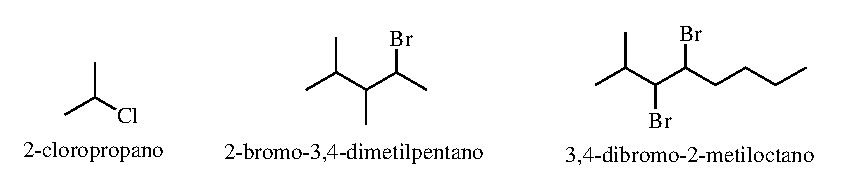
\includegraphics[scale=1]{halogenuros1.eps}
          \end{figure}
    \item También se usan nombres de clase funcional: \ch{CH3Cl} cloruro de metilo (clorometano).
\end{enumerate}

\figura{fig-halogenuros}

\subsection{Alcoholes y fenoles}

Son compuestos derivados de los hidrocarburos en los que se ha sustituido un hidrógeno por un grupo hidroxilo \ch{-OH}. Si el \ch{-OH} está unido a un anillo de benceno el compuesto se llama \blueremark{fenol}.\vspace{6pt}

\mybox{Nomenclatura}

\begin{enumerate}[label=\numberballmDarkTeal]
    \item Se nombran como el hidrocarburo del que proceden, quitando la «o» final y añadiendo la terminación \blueremark{-ol}: etano \(\rightarrow\) etanol. Se indica la posición del grupo \ch{-OH} con el localizador más bajo posible: propan-2-ol.
    \item Si en la molécula hay más de un grupo \ch{-OH}, se utilizan las terminaciones \blueremark{-diol}, \blueremark{-triol}, \blueremark{-tetraol}\dots{} indicando con localizadores las posiciones. En este caso se mantiene la «o» del hidrocarburo: butano-1,2-diol, propano-1,2,3-triol.
    \item La cadena principal es la que contiene el mayor número de grupos \ch{-OH}; si hay empate, la más larga.
    \item Se numera de forma que los grupos \ch{-OH} tengan los localizadores más bajos; el grupo \ch{-OH} tiene preferencia sobre los dobles y triples enlaces: but-3-en-2-ol.
    \item Como siempre, se escriben primero los sustituyentes con su localizador, luego la raíz que indica la longitud de la cadena principal, a continuación las insaturaciones (dobles y triples enlaces), si las hay, y por último la posición y el número de grupos \ch{-OH}.
    \item Si hay un grupo de mayor jerarquía, el grupo \ch{-OH} se nombra como sustituyente con el prefijo \blueremark{hidroxi-}.
\end{enumerate}

\begin{figure}[H]
    \centering
    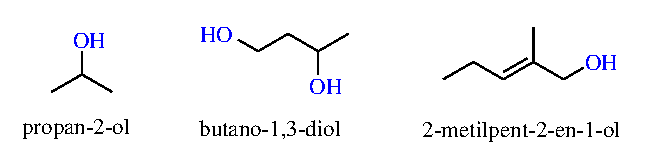
\includegraphics[scale=1]{alcoholes1.eps}
\end{figure}

\figura{fig-alcoholes}


\subsection{Éteres}

Son compuestos que resultan de la unión de dos radicales alquilo o arilo (derivados de un anillo aromático) mediante un átomo de oxígeno, según la estructura general \chemfig{R-O-R'}, siendo R y R\('\) los radicales.\vspace{6pt}

\mybox{Nomenclatura}

\begin{enumerate}[label=\numberballmDarkTeal]
    \item \textbf{Nomenclatura sustitutiva} (es la que prefiere la IUPAC):
          \begin{enumerate}
              \item Se elige el compuesto progenitor R entre los dos radicales con los criterios de siempre: un anillo tiene preferencia sobre una cadena; entre dos cadenas, la más larga; si son igual de largas, la que tiene más enlaces múltiples.
              \item El otro radical, junto con el oxígeno, se nombra como sustituyente quitando la terminación \blueremark{-ano} y añadiendo \blueremark{-oxi}: metoxi, etoxi, propoxi; el de un benceno es fenoxi.
              \item Ejemplos: \ch{CH3-O-CH2-CH3} metoxietano; \ch{C6H5-O-CH3} metoxibenceno.
          \end{enumerate}
    \item \textbf{Nomenclatura de clase funcional} (también admitida): se nombran los dos radicales por orden alfabético seguidos de la palabra \blueremark{éter}, separados por espacios: etil metil éter. Si los dos radicales son iguales se usa el prefijo \blueremark{di-}: dietil éter (o éter dietílico).
\end{enumerate}

\figura{fig-eteres}

\subsection{Aldehídos y cetonas}

Son compuestos que tienen como grupo funcional el grupo carbonilo, \chemfig{>C=O}.
\begin{enumerate}[label=\numberballmDarkTeal]
    \item \textbf{Aldehídos}: el grupo carbonilo está en un carbono terminal, por lo que el carbono del grupo carbonilo está unido al menos a un átomo de hidrógeno (\ch{R-CHO}).
          \begin{figure}[H]
              \centering
              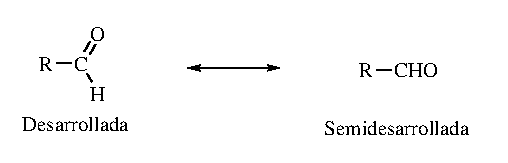
\includegraphics[scale=1]{aldehidos.eps}
          \end{figure}
    \item \textbf{Cetonas}: el grupo carbonilo no está en un carbono terminal y por tanto está unido a dos átomos de carbono: \ch{R-CO-R'}.
          \begin{figure}[H]
              \centering
              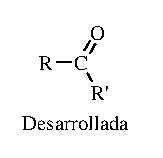
\includegraphics[scale=1]{cetona.eps}
          \end{figure}
\end{enumerate}

\mybox{Nomenclatura}

\begin{enumerate}[label=\numberballmDarkTeal]
    \item \textbf{Aldehídos}
          \begin{enumerate}
              \item Los aldehídos se nombran cambiando la «o» final del hidrocarburo correspondiente por la terminación \blueremark{-al}: propano \(\rightarrow\) propanal.
              \item No es necesario indicar la posición del grupo aldehído, puesto que siempre ocupa una posición terminal: el carbono del grupo \ch{-CHO} es el carbono 1.
              \item Si la molécula tiene dos grupos aldehído (uno en cada extremo), se utiliza la terminación \blueremark{-dial} y se mantiene la «o»: butanodial.
              \item Si el grupo \ch{-CHO} está unido a un anillo, se nombra el anillo seguido de \blueremark{-carbaldehído}: ciclohexanocarbaldehído.
                    \begin{figure}[H]
                        \centering
                        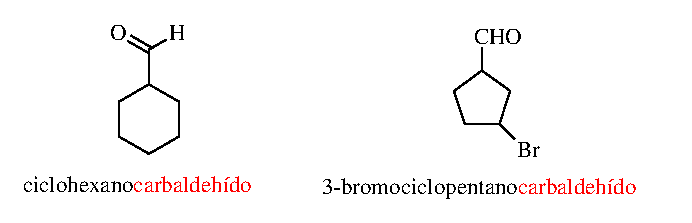
\includegraphics[scale=1]{adehido_2.eps}
                    \end{figure}
              \item Algunos nombres de aldehídos admitidos por la IUPAC son:
                    \begin{figure}[H]
                        \centering
                        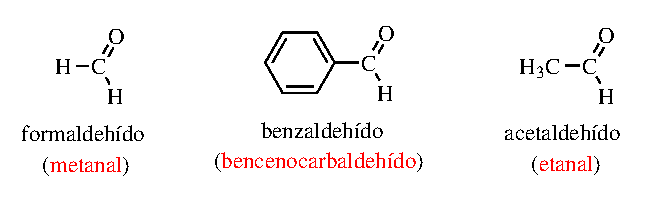
\includegraphics[scale=1]{adehido_3.eps}
                    \end{figure}
              \item Si la cadena principal tiene sustituyentes, estos se nombran delante, seguidos de la raíz que indica el número de átomos de carbono de la cadena principal y la terminación \blueremark{-al}. Si hay alguna insaturación, se indica su posición con su localizador: but-2-enal.
                    \begin{figure}[H]
                        \centering
                        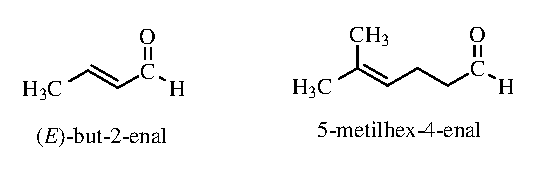
\includegraphics[scale=1]{adehido_4.eps}
                    \end{figure}
              \item Si hay un grupo de mayor jerarquía, el aldehído se nombra como sustituyente: con el prefijo \blueremark{oxo-} si su carbono forma parte de la cadena principal (\ch{=O}) y con el prefijo \blueremark{formil-} si el grupo \ch{-CHO} completo es un sustituyente.
          \end{enumerate}
    \item \textbf{Cetonas}
          \begin{enumerate}
              \item Las cetonas se nombran cambiando la «o» final del hidrocarburo con igual número de carbonos por la terminación \blueremark{-ona}: propanona.
              \item Se toma como cadena principal la más larga que contiene el grupo carbonilo (o el mayor número de grupos carbonilo).
              \item Se numera para que el grupo carbonilo tenga el localizador más bajo: butan-2-ona (en la butanona y en la propanona no hace falta el localizador). Con dos grupos se usa \blueremark{-diona}: pentano-2,4-diona.
              \item También se pueden nombrar con la nomenclatura de clase funcional: se nombran los dos radicales unidos al grupo carbonilo por orden alfabético, separados por espacios, y se termina con la palabra cetona: etil metil cetona (butanona), 3-metilbutil metil cetona (5-metilhexan-2-ona).
              \item Si hay un grupo de mayor jerarquía, se utiliza el prefijo \blueremark{oxo-}: 3-oxobutanal.
          \end{enumerate}
\end{enumerate}

\figura{fig-aldehidos}

\figura{fig-cetonas}

\subsection{Ácidos carboxílicos}

El grupo funcional de los ácidos carboxílicos es el grupo carboxilo, \ch{-COOH}:
\begin{figure}[H]
    \centering
    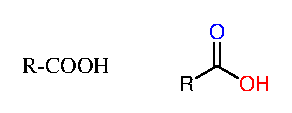
\includegraphics[scale=1]{acido1.eps}
\end{figure}

El grupo carboxilo siempre se encuentra en posición terminal. Se llaman ácidos porque pueden ceder con facilidad el hidrógeno unido al oxígeno (dibujado en color rojo). Es el grupo de mayor jerarquía de los que estudiamos.\vspace{6pt}

\mybox{Nomenclatura}

\begin{enumerate}[label=\numberballmDarkTeal]
    \item Se nombran con la palabra \blueremark{ácido} seguida del nombre del hidrocarburo del que proceden con la terminación \blueremark{-oico}: ácido etanoico.
    \item Si hay dos grupos carboxilo se utiliza la terminación \blueremark{-dioico}: ácido butanodioico.
    \item La cadena principal se empieza a numerar por el extremo donde está el grupo ácido: el carbono del grupo \ch{-COOH} es el carbono 1.
    \item La cadena principal es la que contiene el mayor número de grupos \ch{-COOH}; si hay empate, la más larga.
    \item Si hay dos grupos ácido (uno en cada extremo) y además insaturaciones, se numera de forma que las insaturaciones tengan los localizadores más bajos.
    \item Si hay insaturaciones, se indica su posición con localizadores y se usa la terminación \blueremark{-enoico} para los dobles enlaces o \blueremark{-inoico} para los triples enlaces: ácido but-3-enoico.
    \item Si hay dos o más dobles enlaces tendremos \blueremark{-dienoico}, \blueremark{-trienoico}\dots: ácido hepta-2,4-dienoico.
    \item Si el grupo \ch{-COOH} está unido a un anillo, se usa la terminación \blueremark{-carboxílico}: ácido ciclohexanocarboxílico. Como sustituyente, se usa el prefijo \blueremark{carboxi-}.
    \item Nombres admitidos: ácido fórmico (metanoico), ácido acético (etanoico), ácido benzoico, ácido oxálico (etanodioico).
\end{enumerate}

\figura{fig-acidos}

\subsection{Ésteres}

Se obtienen al sustituir el hidrógeno del grupo \ch{-COOH} de un ácido por un radical R\('\) (reacción de un ácido con un alcohol). Los ésteres tienen el siguiente grupo funcional:

\begin{figure}[H]
    \centering
    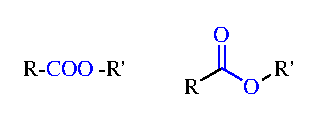
\includegraphics[scale=1]{esteres1.eps}
\end{figure}

\mybox{Nomenclatura}

\begin{enumerate}[label=\numberballmDarkTeal]
    \item Se identifican las dos partes: la que procede del ácido (R--CO--O--) y el radical R\('\) que procede del alcohol.
    \item La cadena principal es la que procede del ácido, es decir, la que está unida al carbono del grupo \ch{-COO-}. El carbono de este grupo se cuenta en la cadena y es el carbono 1.
    \item Se nombran como los ácidos pero quitando la palabra ácido y cambiando la terminación \blueremark{-oico} por \blueremark{-oato}, seguido de la preposición «de» y del nombre del radical R\('\) terminado en \blueremark{-ilo}: etanoato de metilo.
    \item Si hay sustituyentes en las cadenas, en la parte del ácido se numera desde el carbono del grupo \ch{-COO-} y en el radical R\('\) desde el carbono unido al oxígeno.
    \item Si hay alguna insaturación en la cadena principal, se indica su localización con la terminación \blueremark{-enoato} o \blueremark{-inoato}: pent-4-enoato de etilo.
    \item Si el grupo \ch{-COO-} está unido a un anillo se usa \blueremark{-carboxilato}: ciclohexanocarboxilato de metilo. Si hay un grupo de mayor jerarquía, el grupo \ch{-COO-R'} se nombra como prefijo \blueremark{(R\('\))oxicarbonil-}: metoxicarbonil-.
\end{enumerate}

\figura{fig-esteres}

\subsection{Aminas}

Se pueden considerar derivados del amoniaco, \ch{NH3}, en los que se han sustituido uno, dos o tres hidrógenos por radicales orgánicos (alquilos o arilos), dando lugar a aminas primarias (\ch{R-NH2}), secundarias (\ch{R-NH-R'}) y terciarias (\ch{R-N(R')-R''}).\vspace{6pt}

\mybox{Nomenclatura}

\begin{enumerate}[label=\numberballmDarkTeal]
    \item Se nombran añadiendo la terminación \blueremark{-amina} al nombre del hidrocarburo del que proceden (quitando la «o» final), con el localizador que indica la posición del grupo \ch{-NH2}: etanamina, propan-2-amina. También es habitual nombrarlas como el radical seguido de \blueremark{amina}: etilamina, isopropilamina.
    \begin{figure}[H]
        \centering
        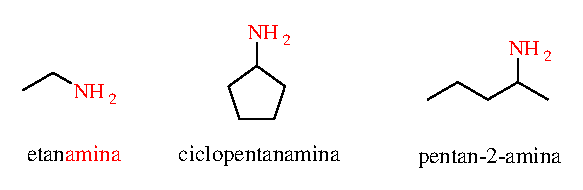
\includegraphics[scale=1]{amina1b.eps}
    \end{figure}

    \item Si un radical está repetido varias veces se indica con los prefijos \blueremark{di-}, \blueremark{tri-}\dots{} Si hay radicales diferentes se nombran por orden alfabético. Los nombres de la figura son tradicionales; los recomendados por la IUPAC son: \recomendado{\textit{N},\textit{N}-dimetilmetanamina, \textit{N}-etil-\textit{N}-metilpropan-1-amina y \textit{N},\textit{N}-dimetilpropan-2-amina}.
    \begin{figure}[H]
        \centering
        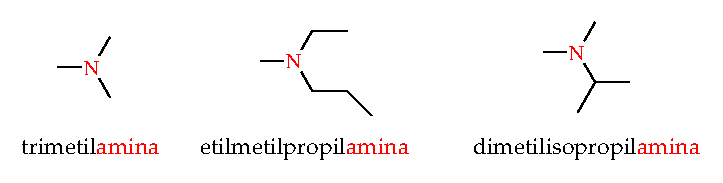
\includegraphics[scale=1]{amina2c.eps}
    \end{figure}

    \item En las aminas secundarias y terciarias se toma como compuesto progenitor el radical más largo (o el anillo); los demás radicales, unidos directamente al nitrógeno, se nombran como sustituyentes con el localizador \blueremark{\textit{N}}: \textit{N}-metiletanamina. Si en la molécula hay dos grupos amino sustituidos se emplea \blueremark{\textit{N},\textit{N}\('\)}.
          \begin{figure}[H]
              \centering
              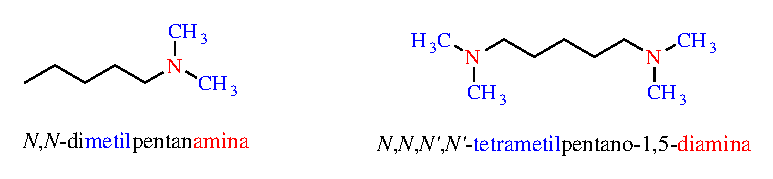
\includegraphics[scale=1]{amina3.eps}
          \end{figure}
    \item Si hay un grupo de mayor jerarquía, el grupo \ch{-NH2} se nombra como sustituyente con el prefijo \blueremark{amino-}: 2-aminoetan-1-ol.
\end{enumerate}

\figura{fig-aminas}

\subsection{Amidas}

Derivan de los ácidos carboxílicos (\ch{R-COOH}) al sustituir el grupo hidroxilo \ch{-OH} por un grupo amino, por lo que su fórmula general es \ch{R}\azul{\ch{CO}}\rojo{\ch{NH2}} o, si el nitrógeno tiene radicales, \ch{R}\azul{\ch{CO}}\rojo{\ch{NR'R''}}.

\begin{figure}[H]
    \centering
    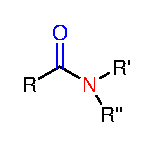
\includegraphics[scale=1]{amida1.eps}
\end{figure}

\mybox{Nomenclatura}

\begin{enumerate}[label=\numberballmDarkTeal]
    \item Se nombran como el hidrocarburo del que proceden (el carbono del grupo \ch{-CO-NH2} también se cuenta para determinar la longitud de la cadena y es el carbono 1), sustituyendo la «o» final por la terminación \blueremark{-amida}: etanamida.
          \begin{figure}[H]
              \centering
              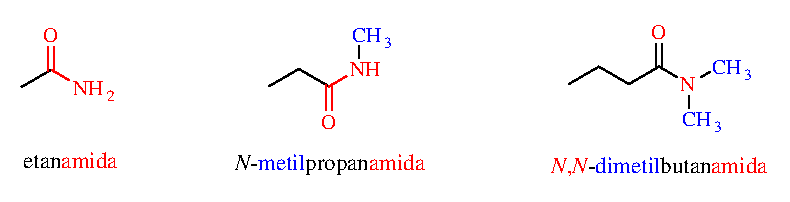
\includegraphics[scale=1]{amida4.eps}
          \end{figure}
    \item Si hay insaturaciones o sustituyentes en la cadena, se indican con localizadores; la cadena empieza a numerarse por el carbono del grupo amida.
    \begin{figure}[H]
        \centering
        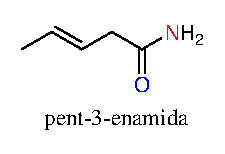
\includegraphics[scale=1]{amida2.eps}
    \end{figure}
    \item Si el nitrógeno del grupo amida tiene algún radical, este se especifica anteponiendo la letra \blueremark{\textit{N}} y se escribe delante del nombre de la amida: \textit{N}-metilpropanamida.
    \begin{figure}[H]
        \centering
        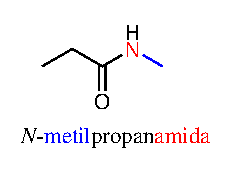
\includegraphics[scale=1]{amida3.eps}
    \end{figure}
    \item Cuando el grupo amida no es el grupo principal y actúa como sustituyente se utiliza el prefijo \blueremark{carbamoil-}.

    \item Si el grupo \ch{-CO-NH2} está unido a un anillo, se nombra el anillo y se termina con el sufijo \blueremark{-carboxamida}: bencenocarboxamida (benzamida), 4-bromo-3-metilciclohexano-1-carboxamida.

\end{enumerate}

\figura{fig-amidas}

\section{Otros grupos de interés}

Otros grupos de interés son:

\subsection{Nitroderivados}

Son compuestos cuyo grupo funcional es:

\begin{figure}[H]
    \centering
    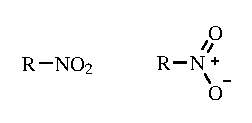
\includegraphics[scale=1]{nitro1.eps}
\end{figure}

\mybox{Nomenclatura}\vspace{6pt}

Se nombran siempre como \textbf{sustituyente}, con el prefijo \blueremark{nitro-}, y nunca como grupo principal.

\begin{figure}[H]
    \centering
    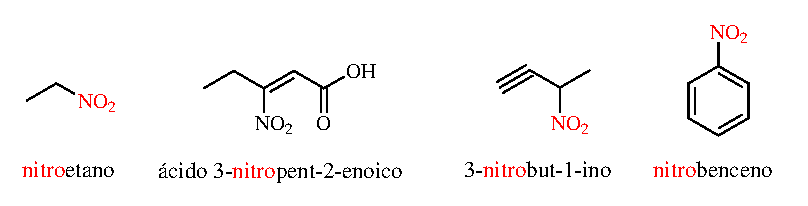
\includegraphics[scale=1]{nitro2.eps}
\end{figure}

\figura{fig-nitro}


\subsection{Nitrilos}

Su grupo funcional es el grupo ciano, \ch{-C+N}:

\begin{figure}[H]
    \centering
    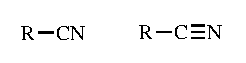
\includegraphics[scale=1]{nitrilo1.eps}
\end{figure}

\mybox{Nomenclatura}

\begin{enumerate}[label=\numberballmDarkTeal]
    \item Cuando actúa como grupo principal se utiliza la terminación \blueremark{-nitrilo} (el carbono del grupo \ch{-C+N} se cuenta en la cadena y es el carbono 1): etanonitrilo. Con dos grupos, \blueremark{-dinitrilo}: butanodinitrilo.
    \item Si el grupo \ch{-C+N} está unido a un anillo se usa la terminación \blueremark{-carbonitrilo}: bencenocarbonitrilo (benzonitrilo).
    \item Cuando actúa como sustituyente se usa el prefijo \blueremark{ciano-}.
\end{enumerate}

\figura{fig-nitrilos}

\section{Compuestos con varios grupos funcionales}

Cuando una molécula tiene varios grupos funcionales distintos se procede así:

\begin{enumerate}[label=\numberballmDarkTeal]
    \item Se busca en la tabla \ref{table:gruposfuncionales2} el grupo de \textbf{mayor jerarquía}: es el grupo principal y se nombra como sufijo.
    \item Se elige la cadena principal que lo contiene y se numera para que tenga el localizador más bajo.
    \item El resto de grupos se nombran como \textbf{prefijos} (hidroxi-, oxo-, amino-, carboxi-\dots), junto con los demás sustituyentes, en orden alfabético.
\end{enumerate}

\figura{fig-polifuncional}

% \newpage{}

% \myemptypage{}

% \newpage{}



\section{Ejercicios}

% Ejercicios de formulación orgánica (se incluye desde organica_apuntes_nuevo.tex).
% Cada ejercicio lleva su solución en un entorno solu: se escribe en ans1.tex
% y se imprime al final del documento.
% En las soluciones, \recomendado{...} indica el nombre según las recomendaciones
% IUPAC 2013 (Guía Breve 2021) cuando no coincide con el nombre tradicional.

\subsection*{Alcanos}

\begin{exercise}
    Formula los siguientes alcanos:
    \begin{multicols}{2}
        \begin{enumerate}[label=\alph*)]
            \item Pentano.
            \item 2,3,4-trimetilheptano.
            \item 4-etil-2,6-dimetiloctano.
            \item 4,6-dietil-2,4,8-trimetilnonano.
            \item 4-etil-2,2,5,8-tetrametil-6-propildecano.
            \item 3,7-dietil-5-isopropildecano.
        \end{enumerate}
    \end{multicols}
    \begin{solu}
        \textcolor{blue}{Se dibuja la cadena principal, se numera y se colocan los sustituyentes en sus posiciones.}
        \begin{enumerate}[label=\alph*)]
            \item \chemfig{CH_3-CH_2-CH_2-CH_2-CH_3} \quad (ya no se usa «n-pentano»)
            \item \chemfig{CH_3-CH(-[2]CH_3)-CH(-[6]CH_3)-CH(-[2]CH_3)-CH_2-CH_2-CH_3}
            \item \chemfig{CH_3-CH(-[2]CH_3)-CH_2-CH(-[6]CH_2-[0]CH_3)-CH_2-CH(-[2]CH_3)-CH_2-CH_3}
            \item \chemfig{CH_3-CH(-[2]CH_3)-CH_2-C(-[2]CH_3)(-[6]CH_2-[0]CH_3)-CH_2-CH(-[6]CH_2-[0]CH_3)-CH_2-CH(-[2]CH_3)-CH_3}
            \item \chemfig{CH_3-C(-[2]CH_3)(-[6]CH_3)-CH_2-CH(-[2]CH_2-[0]CH_3)-CH(-[6]CH_3)-CH(-[2]CH_2-[0]CH_2-[0]CH_3)-CH_2-CH(-[6]CH_3)-CH_2-CH_3}
            \item \chemfig{CH_3-CH_2-CH(-[2]CH_2-[0]CH_3)-CH_2-CH(-[6]CH(-[4]CH_3)-[6]CH_3)-CH_2-CH(-[2]CH_2-[0]CH_3)-CH_2-CH_2-CH_3}\\
                  \recomendado{3,7-dietil-5-(propan-2-il)decano}
        \end{enumerate}
    \end{solu}
\end{exercise}

\begin{exercise}
    Nombra los siguientes alcanos:
    \begin{enumerate}[label=\alph*)]
        \item \chemfig{CH_3-CH(-[2]CH_3)-CH_2-CH(-[6]CH_3)-CH(-[2]CH_3)-CH_3}
        \item \chemfig{CH_3-CH(-[6]CH_3)-CH_2-C(-[2]CH_3)(-[6]CH_3)-CH_2-CH_2-CH_3}
        \item \chemfig{CH_3-CH(-[2]CH_3)-CH(-[6]CH_3)-CH_2-C(-[2]CH_3)(-[6]CH_3)-CH_3}
        \item \chemfig{CH_3-C(-[2]CH_3)(-[6]CH_3)-CH_2-CH(-[6]CH_2-[0]CH_3)-CH(-[2]CH_3)-CH_2-CH(-[6]CH_3)-CH_3}
        \item \chemfig{CH_3-CH_2-CH(-[2]CH_3)-CH(-[6]CH_2-[6]CH_2-[6]CH_3)-CH(-[2]CH_3)-CH(-[6]CH_2-[0]CH_3)-CH(-[2]CH_3)-CH_3}
        \item \chemfig{CH_3-CH_2-C(-[2]CH_3)(-[6]CH(-[4]CH_3)-[6]CH_3)-CH(-[6]CH_3)-CH(-[6]CH_2-[0]CH_3)-CH_2-CH_2-CH_3}
    \end{enumerate}
    \begin{solu}
        \textcolor{blue}{Cadena más larga; si hay varias igual de largas, la de más sustituyentes. Después, localizadores más bajos para el conjunto de sustituyentes.}
        \begin{enumerate}[label=\alph*)]
            \item \textcolor{red}{2,3,5-trimetilhexano} (\{2,3,5\} es más bajo que \{2,4,5\})
            \item \textcolor{red}{2,4,4-trimetilheptano}
            \item \textcolor{red}{2,2,4,5-tetrametilhexano} (se numera desde la derecha: \{2,2,4,5\} es más bajo que \{2,3,5,5\})
            \item \textcolor{red}{4-etil-2,2,5,7-tetrametiloctano}
            \item \textcolor{red}{3-etil-2,4,6-trimetil-5-propiloctano}: hay varias cadenas de 8 carbonos y se elige la que tiene 5 sustituyentes; se numera desde la derecha.
            \item \textcolor{red}{3,5-dietil-2,3,4-trimetiloctano}: la cadena de 8 C que pasa por el grupo isopropilo tiene 5 sustituyentes (la horizontal solo tiene 4).
        \end{enumerate}
    \end{solu}
\end{exercise}

\subsection*{Alquenos y alquinos}

\begin{exercise}
    Formula los siguientes alquenos y alquinos:
    \begin{multicols}{2}
        \begin{enumerate}[label=\alph*)]
            \item But-1-eno.
            \item Pent-2-eno.
            \item Hexa-2,4-dieno.
            \item 3-butilhexa-1,4-dieno.
            \item But-2-ino.
            \item 3,4-dimetilpent-1-ino.
            \item 3,6-dimetilnona-1,4,7-triino.
            \item Pent-1-en-3-ino.
            \item Hept-3-en-1,6-diino.
            \item 4-etilhexa-1,3-dien-5-ino.
        \end{enumerate}
    \end{multicols}
    \begin{solu}
        \begin{enumerate}[label=\alph*)]
            \item \chemfig{CH_2=CH-CH_2-CH_3}
            \item \chemfig{CH_3-CH=CH-CH_2-CH_3}
            \item \chemfig{CH_3-CH=CH-CH=CH-CH_3}
            \item \chemfig{CH_2=CH-CH(-[6]CH_2-[0]CH_2-[0]CH_2-[0]CH_3)-CH=CH-CH_3}\\
                  \recomendado{4-eteniloct-2-eno}: la cadena más larga (8 C) pasa por el grupo butilo, aunque tenga un doble enlace menos.
            \item \chemfig{CH_3-C~C-CH_3}
            \item \chemfig{CH~C-CH(-[2]CH_3)-CH(-[6]CH_3)-CH_3}
            \item \chemfig{CH~C-CH(-[2]CH_3)-C~C-CH(-[2]CH_3)-C~C-CH_3}
            \item \chemfig{CH_2=CH-C~C-CH_3}
            \item \chemfig{CH~C-CH=CH-CH_2-C~CH} \quad (\{1,3,6\} es más bajo que \{1,4,6\})
            \item \chemfig{CH_2=CH-CH=C(-[6]CH_2-[0]CH_3)-C~CH} \quad (empate \{1,3,5\}: los dobles enlaces reciben 1 y 3)
        \end{enumerate}
    \end{solu}
\end{exercise}

\begin{exercise}
    Nombra los siguientes alquenos y alquinos:
    \begin{enumerate}[label=\alph*)]
        \item \chemfig{CH_3-CH=CH-CH_2-CH_2-CH_3}
        \item \chemfig{CH_2=CH-C(-[6]CH_3)=CH-CH_3}
        \item \chemfig{CH~C-CH(-[6]CH_3)-CH_2-CH_3}
        \item \chemfig{CH_3-CH=C(-[6]CH_3)-CH_2-CH_3}
        \item \chemfig{CH~C-C~C-CH_2-CH_3}
        \item \chemfig{CH~C-CH=CH-CH_3}
        \item \chemfig{CH_2=CH-CH(-[6]CH_3)-CH_2-CH_2-C~CH}
        \item \chemfig{CH_3-CH=C(-[6]CH_3)-CH_2-C~C-CH(-[2]CH_3)-CH=CH_2}
        \item \chemfig{CH_2=CH-CH(-[6]CH(-[6]CH_3)-CH_3)-CH_2-C~C-CH(-[6]CH_2-[6]CH_3)-C~CH}
    \end{enumerate}
    \begin{solu}
        \textcolor{blue}{Localizadores más bajos para el conjunto de dobles y triples enlaces; si hay empate, para los dobles.}
        \begin{enumerate}[label=\alph*)]
            \item \textcolor{red}{hex-2-eno}
            \item \textcolor{red}{3-metilpenta-1,3-dieno}
            \item \textcolor{red}{3-metilpent-1-ino}
            \item \textcolor{red}{3-metilpent-2-eno}
            \item \textcolor{red}{hexa-1,3-diino}
            \item \textcolor{red}{pent-3-en-1-ino} (\{1,3\} es más bajo que \{2,4\})
            \item \textcolor{red}{3-metilhept-1-en-6-ino} (empate \{1,6\}: el doble enlace recibe el 1)
            \item \textcolor{red}{3,7-dimetilnona-1,7-dien-4-ino} (se numera desde la derecha: \{1,4,7\})
            \item \textcolor{red}{3-etil-7-isopropilnon-8-en-1,4-diino}, \recomendado{3-etil-7-(propan-2-il)non-8-en-1,4-diino}. Todas las cadenas posibles tienen 9 C; se elige la que tiene más enlaces múltiples y se numera desde la derecha (\{1,4,8\}).
        \end{enumerate}
    \end{solu}
\end{exercise}

\subsection*{Hidrocarburos cíclicos}

\begin{exercise}
    Formula los siguientes hidrocarburos cíclicos:
    \begin{multicols}{2}
        \begin{enumerate}[label=\alph*)]
            \item Etilciclohexano.
            \item Ciclopenteno.
            \item Ciclohexino.
            \item 1,1,4,4-tetrametilciclohexano.
            \item 3-etilciclopenteno.
            \item 1,6-dimetilciclohexeno.
            \item 4-ciclobutilpent-1-ino.
            \item 3-ciclohexil-5-metilhex-2-eno.
            \item Ciclohexa-1,3-dieno.
            \item 3-ciclopentilprop-1-eno.
        \end{enumerate}
    \end{multicols}
    \begin{solu}
        \begin{enumerate}[label=\alph*)]
            \item \chemfig{*6(---(-CH_2-[0]CH_3)---)}
            \item \chemfig{*5(=----)}
            \item \chemfig{*6(~-----)}
            \item \chemfig{*6(-(-[::30]CH_3)(-[::-30]CH_3)---(-[::30]CH_3)(-[::-30]CH_3)--)}
            \item \chemfig{*5(=-(-CH_2-CH_3)---)}
            \item \chemfig{*6(-=(-CH_3)-(-CH_3)---)}\\
                  Los carbonos del doble enlace son el 1 y el 2; \{1,6\} es más bajo que \{2,3\}, por eso no se dice \mal{2,3-dimetilciclohexeno}.
            \item \chemfig{CH~C-CH_2-CH(-[6]*4(----))-CH_3}\\
                  \recomendado{(pent-4-in-2-il)ciclobutano}: el anillo tiene preferencia sobre la cadena.
            \item \chemfig{CH_3-CH=C(-[6]*6(------))-CH_2-CH(-[2]CH_3)-CH_3}\\
                  \recomendado{(5-metilhex-2-en-3-il)ciclohexano}
            \item \chemfig{*6(=-=---)}
            \item \chemfig{CH_2=CH-CH_2-[0]*5(-----)}\\
                  \recomendado{(prop-2-en-1-il)ciclopentano} o alilciclopentano
        \end{enumerate}
    \end{solu}
\end{exercise}

\begin{exercise}
    Nombra los siguientes hidrocarburos:
    \begin{enumerate}[label=\alph*)]
        \item \chemfig{*4(----)}
        \item \chemfig{*6(-----=)}
        \item \chemfig{*6(---(-CH_3)--(-CH_2-[2]CH_3)-)}
        \item \chemfig{*6(---=-=)}
        \item \chemfig{*6(---(-CH(-[:50]CH_3)(-[:-50]CH_3))---)}
        \item \chemfig{CH_3-CH(-[6]*6(------))-CH_2-CH_2-C(-[2]CH_3)(-[6]CH_3)-CH_2-CH_3}
        \item \chemfig{CH_3-CH(-[6]*5(-----))-CH=CH_2}
    \end{enumerate}
    \begin{solu}
        \begin{enumerate}[label=\alph*)]
            \item \textcolor{red}{ciclobutano}
            \item \textcolor{red}{ciclohexeno}
            \item \textcolor{red}{1-etil-3-metilciclohexano} (empate \{1,3\}: etil va antes por orden alfabético)
            \item \textcolor{red}{ciclohexa-1,3-dieno}
            \item \textcolor{red}{isopropilciclohexano}, \recomendado{(propan-2-il)ciclohexano}
            \item \textcolor{red}{2-ciclohexil-5,5-dimetilheptano}, \recomendado{(5,5-dimetilheptan-2-il)ciclohexano}
            \item \textcolor{red}{3-ciclopentilbut-1-eno}, \recomendado{(but-3-en-2-il)ciclopentano}
        \end{enumerate}
    \end{solu}
\end{exercise}

\subsection*{Hidrocarburos aromáticos}

\begin{exercise}
    Formula los siguientes hidrocarburos aromáticos:
    \begin{multicols}{2}
        \begin{enumerate}[label=\alph*)]
            \item Metilbenceno (tolueno).
            \item 1,3-dietilbenceno.
            \item Etenilbenceno (estireno).
            \item 1-butil-4-isopropilbenceno.
            \item \textit{p}-propiltolueno.
            \item 3-fenil-5-metilheptano.
            \item 4-fenilpent-1-eno.
            \item 2,4-difenil-3-metilhexano.
        \end{enumerate}
    \end{multicols}
    \begin{solu}
        \begin{enumerate}[label=\alph*)]
            \item \chemfig{CH_3-**6(------)}
            \item \chemfig{**6(-(-CH_2-CH_3)--(-CH_2-CH_3)---)}
            \item \chemfig{CH_2=CH-**6(------)}
            \item \chemfig{CH_3-CH_2-CH_2-CH_2-**6(---(-CH(-[2]CH_3)-CH_3)---)}\\
                  \recomendado{1-butil-4-(propan-2-il)benceno}
            \item \chemfig{CH_3-**6(---(-CH_2-CH_2-CH_3)---)}: \textcolor{red}{1-metil-4-propilbenceno}
            \item \chemfig{CH_3-CH_2-CH(-[6]**6(------))-CH_2-CH(-[2]CH_3)-CH_2-CH_3}\\
                  \recomendado{(5-metilheptan-3-il)benceno}
            \item \chemfig{CH_2=CH-CH_2-CH(-[6]**6(------))-CH_3}\\
                  \recomendado{(pent-4-en-2-il)benceno}
            \item \chemfig{CH_3-CH(-[6]**6(------))-CH(-[2]CH_3)-CH(-[6]**6(------))-CH_2-CH_3}\\
                  \recomendado{1,1\('\)-(3-metilhexano-2,4-diil)dibenceno}
        \end{enumerate}
    \end{solu}
\end{exercise}

\begin{exercise}
    Nombra los siguientes hidrocarburos aromáticos:
    \begin{enumerate}[label=\alph*)]
        \item \chemfig{CH_3-CH(-[6]**6(------))-CH_2-C(-[2]CH_3)(-[6]CH_3)-CH_3}
        \item \chemfig{**6(----(-CH_2-[:0]CH_3)--)}
        \item \chemfig{**6(-(-CH_2-CH_2-CH_3)--(-CH_3)---)}
        \item \chemfig{**6(-(-CH_3)--(-CH_3)--(-CH_3)-)}
        \item \chemfig{**6(----(-CH(-[1]CH_3)(-[3]H_3C))--)}
        \item \chemfig{**6(--(-[:0]CH_2-[:0]CH_2-[:0]CH_2-[:0]**6(------))----)}
        \item \chemfig{CH_3-CH=C(-[6]**6(------))-CH_2-CH_3}
    \end{enumerate}
    \begin{solu}
        \begin{enumerate}[label=\alph*)]
            \item \textcolor{red}{2,2-dimetil-4-fenilpentano}, \recomendado{(4,4-dimetilpentan-2-il)benceno}
            \item \textcolor{red}{etilbenceno}
            \item \textcolor{red}{1-metil-3-propilbenceno} (\textit{m}-propiltolueno)
            \item \textcolor{red}{1,3,5-trimetilbenceno}
            \item \textcolor{red}{isopropilbenceno} (cumeno), \recomendado{(propan-2-il)benceno}
            \item \textcolor{red}{1,3-difenilpropano}, \recomendado{1,1\('\)-(propano-1,3-diil)dibenceno}
            \item \textcolor{red}{3-fenilpent-2-eno}, \recomendado{(pent-2-en-3-il)benceno}
        \end{enumerate}
    \end{solu}
\end{exercise}

\subsection*{Derivados halogenados}

\begin{exercise}
    Formula los siguientes derivados halogenados:
    \begin{multicols}{2}
        \begin{enumerate}[label=\alph*)]
            \item 2-cloropropano.
            \item 1,3-dibromobenceno.
            \item 1,1,2,2-tetrafluoroetano.
            \item 1,4-diclorociclohexano.
            \item 4-bromopent-1-ino.
            \item 3-fluoro-5-metilhex-2-eno.
            \item 1,4-dibromo-6-ciclopentiloct-2-eno.
            \item 2,5-difenil-4-yodopent-1-eno.
            \item 4-clorobut-1-eno.
            \item 1,2-dibromobenceno.
        \end{enumerate}
    \end{multicols}
    \begin{solu}
        \begin{enumerate}[label=\alph*)]
            \item \chemfig{CH_3-CH(-[2]Cl)-CH_3}
            \item \chemfig{**6(-(-Br)--(-Br)---)}
            \item \chemfig{CHF_2-CHF_2}
            \item \chemfig{*6(-(-Cl)---(-Cl)--)}
            \item \chemfig{CH~C-CH_2-CH(-[2]Br)-CH_3}
            \item \chemfig{CH_3-CH=C(-[2]F)-CH_2-CH(-[2]CH_3)-CH_3}
            \item \chemfig{CH_2(-[2]Br)-CH=CH-CH(-[2]Br)-CH_2-CH(-[6]*5(-----))-CH_2-CH_3}\\
                  \recomendado{(5,8-dibromooct-6-en-3-il)ciclopentano}
            \item \chemfig{CH_2=C(-[2]**6(------))-CH_2-CH(-[6]I)-CH_2-[0]**6(------)}
            \item \chemfig{CH_2=CH-CH_2-CH_2-Cl}
            \item \chemfig{**6(-(-Br)-(-Br)----)}
        \end{enumerate}
    \end{solu}
\end{exercise}

\begin{exercise}
    Nombra los siguientes derivados halogenados:
    \begin{enumerate}[label=\alph*)]
        \item \chemfig{CH_3-I}
        \item \chemfig{CH_2(-[2]Cl)-CH_2(-[6]Cl)}
        \item \chemfig{CH_3-C(-[2]Br)(-[6]Br)-CH_2-CH_3}
        \item \chemfig{CH_2(-[2]Cl)-CH_2-CH=CH_2}
        \item \chemfig{CH~C-CH(-[2]Br)-CH_2-CH_2-Br}
        \item \chemfig{**6(----(-F)--)}
        \item \chemfig{CH_3-CH(-[2]Cl)-CH_2-CH_2-[0]*4(----)}
        \item \chemfig{*6(-(-Br)--(-Br)---)}
        \item \chemfig{CH_2(-[4]F)-CH(-[2]F)(-[6]F)}
        \item \chemfig{*5(-(-Cl)---(-Cl)-)}
    \end{enumerate}
    \begin{solu}
        \begin{enumerate}[label=\alph*)]
            \item \textcolor{red}{yodometano}
            \item \textcolor{red}{1,2-dicloroetano}
            \item \textcolor{red}{2,2-dibromobutano}
            \item \textcolor{red}{4-clorobut-1-eno} (el doble enlace se numera antes que el halógeno)
            \item \textcolor{red}{3,5-dibromopent-1-ino}
            \item \textcolor{red}{fluorobenceno}
            \item \textcolor{red}{1-ciclobutil-3-clorobutano}, \recomendado{(3-clorobutil)ciclobutano}
            \item \textcolor{red}{1,3-dibromociclohexano}
            \item \textcolor{red}{1,1,2-trifluoroetano}
            \item \textcolor{red}{1,3-diclorociclopentano}
        \end{enumerate}
    \end{solu}
\end{exercise}

\subsection*{Alcoholes y éteres}

\begin{exercise}
    Formula los siguientes alcoholes y éteres:
    \begin{multicols}{2}
        \begin{enumerate}[label=\alph*)]
            \item 3-metilpentan-1-ol.
            \item Butano-1,2,3-triol.
            \item 2-fenilpropano-1,3-diol.
            \item Ciclohexanol.
            \item Hexa-3,5-dien-2-ol.
            \item Fenol (bencenol).
            \item 2-etilpentan-1-ol.
            \item Pent-3-en-1-ol.
            \item Etil isopropil éter.
            \item Etenil fenil éter.
            \item Dimetil éter.
            \item Butil ciclopentil éter.
        \end{enumerate}
    \end{multicols}
    \begin{solu}
        \begin{enumerate}[label=\alph*)]
            \item \chemfig{CH_2(-[2]OH)-CH_2-CH(-[2]CH_3)-CH_2-CH_3}
            \item \chemfig{CH_2(-[2]OH)-CH(-[2]OH)-CH(-[2]OH)-CH_3}
            \item \chemfig{CH_2(-[2]OH)-CH(-[6]**6(------))-CH_2(-[2]OH)}
            \item \chemfig{*6(---(-OH)---)}
            \item \chemfig{CH_3-CH(-[2]OH)-CH=CH-CH=CH_2}
            \item \chemfig{**6(---(-OH)---)}
            \item \chemfig{CH_2(-[2]OH)-CH(-[6]CH_2-[0]CH_3)-CH_2-CH_2-CH_3}
            \item \chemfig{CH_2(-[2]OH)-CH_2-CH=CH-CH_3}
            \item \chemfig{CH_3-CH_2-O-CH(-[2]CH_3)-CH_3}: \recomendado{2-etoxipropano}
            \item \chemfig{CH_2=CH-O-**6(------)}: \recomendado{(eteniloxi)benceno}
            \item \chemfig{CH_3-O-CH_3}: \recomendado{metoximetano}
            \item \chemfig{CH_3-CH_2-CH_2-CH_2-O-*5(-----)}: \recomendado{butoxiciclopentano} (el anillo es el progenitor)
        \end{enumerate}
    \end{solu}
\end{exercise}

\begin{exercise}
    Nombra los siguientes alcoholes y éteres:
    \begin{enumerate}[label=\alph*)]
        \item \chemfig{CH_3-OH}
        \item \chemfig{CH_2(-[2]OH)-CH_2-CH(-[6]CH_2-[0]CH_3)-CH=CH_2}
        \item \chemfig{CH_3-CH(-[2]OH)-CH(-[6]Br)-CH_2(-[2]OH)}
        \item \chemfig{CH_3-CH_2-CH(-[2]CH_3)-CH(-[6]CH_3)-CH(-[2]OH)-CH=CH_2}
        \item \chemfig{CH_2=CH-CH(-[2]OH)-CH_2(-[2]OH)}
        \item \chemfig{CH_3-CH_2-CH_2-O-CH_2-CH_2-CH_3}
        \item \chemfig{CH_2=CH-O-CH(-[2]CH_3)-CH_3}
        \item \chemfig{CH_3-CH_2-CH_2-CH_2-CH_2-O-C~CH}
    \end{enumerate}
    \begin{solu}
        \begin{enumerate}[label=\alph*)]
            \item \textcolor{red}{metanol}
            \item \textcolor{red}{3-etilpent-4-en-1-ol}: las dos cadenas que contienen el \ch{-OH} tienen 5 C; se elige la que tiene el doble enlace.
            \item \textcolor{red}{2-bromobutano-1,3-diol}
            \item \textcolor{red}{4,5-dimetilhept-1-en-3-ol}: el \ch{-OH} recibe el localizador más bajo (3).
            \item \textcolor{red}{but-3-eno-1,2-diol}
            \item \textcolor{red}{dipropil éter}, \recomendado{1-propoxipropano}
            \item \textcolor{red}{etenil isopropil éter}, \recomendado{2-(eteniloxi)propano}: el propano (3 C) es más largo que el eteno.
            \item \textcolor{red}{etinil pentil éter}, \recomendado{1-(etiniloxi)pentano}
        \end{enumerate}
    \end{solu}
\end{exercise}

\subsection*{Aldehídos y cetonas}

\begin{exercise}
    Formula los siguientes aldehídos y cetonas:
    \begin{multicols}{2}
        \begin{enumerate}[label=\alph*)]
            \item Etanal (acetaldehído).
            \item 3-metilpentanal.
            \item Propenal.
            \item 5-ciclohexilpent-3-inal.
            \item Hex-2-enodial.
            \item Hexano-2,4-diona.
            \item 1,4-difenilpentan-2-ona.
            \item Benzaldehído.
            \item 2-metilpentanodial.
            \item 3-metilpent-2-enal.
            \item Pentan-2-ona.
            \item 3-clorobutan-2-ona.
            \item Hexa-1,5-dien-3-ona.
        \end{enumerate}
    \end{multicols}
    \begin{solu}
        \begin{enumerate}[label=\alph*)]
            \item \chemfig{CH_3-!{aldehido}}
            \item \chemfig{CH_3-CH_2-CH(-[2]CH_3)-CH_2-!{aldehido}}
            \item \chemfig{CH_2=CH-!{aldehido}} (prop-2-enal)
            \item \chemfig{!{aldehido2}-CH_2-C~C-CH_2-[0]*6(------)}
            \item \chemfig{!{aldehido2}-CH=CH-CH_2-CH_2-!{aldehido}}
            \item \chemfig{CH_3-C(=[2]O)-CH_2-C(=[2]O)-CH_2-CH_3} (no «hexa-»: no tiene dobles enlaces C=C)
            \item \chemfig{CH_3-CH(-[6]**6(------))-CH_2-C(=[2]O)-CH_2-[0]**6(------)}
            \item \chemfig{**6(---(-CHO)---)}
            \item \chemfig{!{aldehido2}-CH(-[6]CH_3)-CH_2-CH_2-!{aldehido}}
            \item \chemfig{CH_3-CH_2-C(-[6]CH_3)=CH-!{aldehido}}
            \item \chemfig{CH_3-C(=[2]O)-CH_2-CH_2-CH_3}
            \item \chemfig{CH_3-C(=[2]O)-CH(-[2]Cl)-CH_3}
            \item \chemfig{CH_2=CH-C(=[2]O)-CH_2-CH=CH_2}
        \end{enumerate}
    \end{solu}
\end{exercise}

\begin{exercise}
    Nombra los siguientes aldehídos y cetonas:
    \begin{enumerate}[label=\alph*)]
        \item \chemfig{H-!{aldehido}}
        \item \chemfig{CH_3-CH_2-CH_2-!{aldehido}}
        \item \chemfig{!{aldehido2}-CH=CH-!{aldehido}}
        \item \chemfig{CH_2=C(-[6]!{fenil})-CH_2-CH_2-!{aldehido}}
        \item \chemfig{!{aldehido2}-CH=CH-CH_2-CH(-[2]CH_3)-!{aldehido}}
        \item \chemfig{CH_3-CH(-[6]!{fenil})-CH=CH-!{aldehido}}
        \item \chemfig{!{aldehido2}-CH_2-C~C-CH_2-CH_2-!{aldehido}}
        \item \chemfig{CH_3-C(=[2]O)-CH_2-CH_3}
        \item \chemfig{CH_3-CH=CH-CH_2-C(=[2]O)-CH_3}
        \item \chemfig{CH_3-C(=[2]O)-CH_2-CH_2-CH_2-C(=[2]O)-CH_3}
        \item \chemfig{CH_3-CH(-[2]CH_3)-C(=[6]O)-CH_2-CH(-[2]CH_3)-CH_3}
        \item \chemfig{CH_2=CH-C(=[2]O)-CH=CH-CH_3}
    \end{enumerate}
    \begin{solu}
        \begin{enumerate}[label=\alph*)]
            \item \textcolor{red}{metanal} (formaldehído)
            \item \textcolor{red}{butanal}
            \item \textcolor{red}{but-2-enodial}
            \item \textcolor{red}{4-fenilpent-4-enal}
            \item \textcolor{red}{5-metilhex-2-enodial}: los dos \ch{-CHO} dan 1 y 6 en ambos sentidos; decide el doble enlace (2 mejor que 4).
            \item \textcolor{red}{4-fenilpent-2-enal}
            \item \textcolor{red}{hept-3-inodial}
            \item \textcolor{red}{butanona} (butan-2-ona, etil metil cetona)
            \item \textcolor{red}{hex-4-en-2-ona}
            \item \textcolor{red}{heptano-2,6-diona}
            \item \textcolor{red}{2,5-dimetilhexan-3-ona}
            \item \textcolor{red}{hexa-1,4-dien-3-ona}
        \end{enumerate}
    \end{solu}
\end{exercise}

\subsection*{Ácidos carboxílicos y ésteres}

\begin{exercise}
    Formula los siguientes ácidos y ésteres:
    \begin{multicols}{2}
        \begin{enumerate}[label=\alph*)]
            \item Ácido etanoico (ácido acético).
            \item Ácido 3-metilhexanoico.
            \item Ácido 2-fenilpentanodioico.
            \item Ácido tricloroetanoico.
            \item Ácido but-3-enoico.
            \item Ácido hepta-2,4-dienoico.
            \item Ácido pent-2-enodioico.
            \item Ácido benzoico.
            \item Butanoato de metilo.
            \item Propanoato de etilo.
            \item Benzoato de propilo.
            \item Etanoato de octilo.
            \item 3-cloropentanoato de etenilo.
            \item But-3-enoato de isopropilo.
        \end{enumerate}
    \end{multicols}
    \begin{solu}
        \begin{enumerate}[label=\alph*)]
            \item \chemfig{CH_3-!{acido}}
            \item \chemfig{CH_3-CH_2-CH_2-CH(-[2]CH_3)-CH_2-!{acido}}
            \item \chemfig{!{acido2}-CH(-[6]**6(------))-CH_2-CH_2-!{acido}}
            \item \chemfig{CCl_3-!{acido}}
            \item \chemfig{CH_2=CH-CH_2-!{acido}}
            \item \chemfig{CH_3-CH_2-CH=CH-CH=CH-!{acido}}
            \item \chemfig{!{acido2}-CH=CH-CH_2-!{acido}}
            \item \chemfig{**6(---(-COOH)---)}
            \item \chemfig{CH_3-CH_2-CH_2-C(=[2]O)-O-CH_3}
            \item \chemfig{CH_3-CH_2-C(=[2]O)-O-CH_2-CH_3}
            \item \chemfig{CH_3-CH_2-CH_2-O-C(=[2]O)-**6(------)}
            \item \ch{CH3-COO-(CH2)7-CH3}
            \item \chemfig{CH_3-CH_2-CH(-[2]Cl)-CH_2-C(=[2]O)-O-CH=CH_2}
            \item \chemfig{CH_2=CH-CH_2-C(=[2]O)-O-CH(-[2]CH_3)-CH_3}\\
                  \recomendado{but-3-enoato de propan-2-ilo}
        \end{enumerate}
    \end{solu}
\end{exercise}

\begin{exercise}
    Nombra los siguientes ácidos y ésteres:
    \begin{enumerate}[label=\alph*)]
        \item \chemfig{CH_3-CH_2-CH_2-!{acido}}
        \item \chemfig{!{acido2}-CH_2-CH_2-!{acido}}
        \item \chemfig{CH_3-CH=CH-CH_2-!{acido}}
        \item \chemfig{CH_3-CH(-[2]CH_3)-CH_2-CH(-[2]CH_3)-CH_2-!{acido}}
        \item \chemfig{!{acido2}-C~C-CH_2-!{acido}}
        \item \chemfig{CH_3-CH_2-CH(-[6]!{ciclopentil})-!{acido}}
        \item \chemfig{CH_3-C(=[2]O)-O-CH_3}
        \item \chemfig{CH_3-CH_2-CH_2-C(=[2]O)-O-CH_2-CH_3}
        \item \chemfig{CH_3-CH_2-CH_2-CH_2-CH_2-CH_2-CH_2-C(=[2]O)-O-CH_2-CH_2-CH_3}
        \item \chemfig{CH_3-CH_2-CH_2-CH_2-CH_2-C(=[2]O)-O-CH_3}
        \item \chemfig{CH_3-CH(-[2]Br)-CH_2-C(=[2]O)-O-CH=CH_2}
        \item \chemfig{CH_2(-[:180]!{fenil})-CH_2-C(=[2]O)-O-CH_2-CH_2-CH_2-CH_2-CH_2-CH_3}
    \end{enumerate}
    \begin{solu}
        \textcolor{blue}{El carbono del grupo \ch{-COOH} (o \ch{-COO-}) es siempre el carbono 1.}
        \begin{enumerate}[label=\alph*)]
            \item \textcolor{red}{ácido butanoico}
            \item \textcolor{red}{ácido butanodioico} (ácido succínico)
            \item \textcolor{red}{ácido pent-3-enoico}
            \item \textcolor{red}{ácido 3,5-dimetilhexanoico}
            \item \textcolor{red}{ácido pent-2-inodioico}
            \item \textcolor{red}{ácido 2-ciclopentilbutanoico} (el \ch{-COOH} está en la cadena: la cadena es el progenitor)
            \item \textcolor{red}{etanoato de metilo} (acetato de metilo)
            \item \textcolor{red}{butanoato de etilo}
            \item \textcolor{red}{octanoato de propilo}
            \item \textcolor{red}{hexanoato de metilo}
            \item \textcolor{red}{3-bromobutanoato de etenilo} (de vinilo)
            \item \textcolor{red}{3-fenilpropanoato de hexilo}
        \end{enumerate}
    \end{solu}
\end{exercise}

\subsection*{Compuestos nitrogenados}

\begin{exercise}
    Formula los siguientes compuestos nitrogenados:
    \begin{multicols}{2}
        \begin{enumerate}[label=\alph*)]
            \item Isopropilamina.
            \item Pentan-3-amina.
            \item Butano-1,3-diamina.
            \item Etano-1,2-diamina.
            \item 3-etilhexan-3-amina.
            \item 3,5-dimetilhexan-1-amina.
            \item Pent-3-en-2-amina.
            \item \textit{N}-etil-\textit{N}-metilpropan-1-amina.
            \item \textit{N}-metilanilina.
            \item \textit{N}-ciclopentilbutan-1-amina.
            \item Etanamida.
            \item \textit{N}-metiletanamida.
            \item 4-fenilpentanamida.
            \item \textit{N}-etilhex-4-enamida.
        \end{enumerate}
    \end{multicols}
    \begin{solu}
        \begin{enumerate}[label=\alph*)]
            \item \chemfig{CH_3-CH(-[2]NH_2)-CH_3}: \recomendado{propan-2-amina}
            \item \chemfig{CH_3-CH_2-CH(-[2]NH_2)-CH_2-CH_3}
            \item \chemfig{CH_2(-[2]NH_2)-CH_2-CH(-[2]NH_2)-CH_3}
            \item \chemfig{H_2N-CH_2-CH_2-NH_2}
            \item \chemfig{CH_3-CH_2-C(-[2]NH_2)(-[6]CH_2-[0]CH_3)-CH_2-CH_2-CH_3}
            \item \chemfig{H_2N-CH_2-CH_2-CH(-[2]CH_3)-CH_2-CH(-[2]CH_3)-CH_3}
            \item \chemfig{CH_3-CH(-[2]NH_2)-CH=CH-CH_3}
            \item \chemfig{CH_3-CH_2-CH_2-N(-[2]CH_3)-CH_2-CH_3}
            \item \chemfig{**6(---(-NH-CH_3)---)}: \recomendado{\textit{N}-metilanilina} (\textit{N}-metilbencenamina)
            \item \chemfig{CH_3-CH_2-CH_2-CH_2-NH-[0]*5(-----)}: \recomendado{\textit{N}-butilciclopentanamina} (el anillo es el progenitor)
            \item \chemfig{CH_3-C(=[2]O)-NH_2}
            \item \chemfig{CH_3-C(=[2]O)-NH-CH_3}
            \item \chemfig{CH_3-CH(-[6]**6(------))-CH_2-CH_2-C(=[2]O)-NH_2}
            \item \chemfig{CH_3-CH=CH-CH_2-CH_2-C(=[2]O)-NH-CH_2-CH_3}
        \end{enumerate}
    \end{solu}
\end{exercise}

\begin{exercise}
    Nombra los siguientes compuestos nitrogenados:
    \begin{enumerate}[label=\alph*)]
        \item \chemfig{CH_3-CH(-[6]NH_2)-CH_2-CH_3}
        \item \chemfig{CH_3-CH_2-CH_2-NH_2}
        \item \chemfig{CH_3-CH(-[6]NH_2)-CH_2-CH(-[6]NH_2)-CH_2-CH_2-NH_2}
        \item \chemfig{CH_3-CH(-[6]CH_3)-NH-CH=CH_2}
        \item \chemfig{CH_3-CH_2-CH_2-CH_2-CH_2-C(=[2]O)-NH_2}
        \item \chemfig{CH_3-CH_2-C(=[2]O)-N(-[6]CH_3)-CH_3}
        \item \chemfig{CH_3-CH=CH-CH_2-C(=[2]O)-NH_2}
        \item \chemfig{CH_3-CH_2-CH(-[2]Br)-CH_2-CH_2-C(=[2]O)-NH-CH_3}
    \end{enumerate}
    \begin{solu}
        \begin{enumerate}[label=\alph*)]
            \item \textcolor{red}{butan-2-amina}
            \item \textcolor{red}{propan-1-amina} (propilamina)
            \item \textcolor{red}{hexano-1,3,5-triamina} (se numera desde la derecha: \{1,3,5\})
            \item \textcolor{red}{\textit{N}-etenilpropan-2-amina}: el propano (3 C) es más largo que el eteno.
            \item \textcolor{red}{hexanamida}
            \item \textcolor{red}{\textit{N},\textit{N}-dimetilpropanamida}
            \item \textcolor{red}{pent-3-enamida}
            \item \textcolor{red}{4-bromo-\textit{N}-metilhexanamida}
        \end{enumerate}
    \end{solu}
\end{exercise}

\subsection*{Nitrilos y nitroderivados}

\begin{exercise}
    Formula los siguientes compuestos:
    \begin{multicols}{2}
        \begin{enumerate}[label=\alph*)]
            \item Butanonitrilo.
            \item Benzonitrilo.
            \item 2-metilpropanonitrilo.
            \item Nitrobenceno.
            \item 2-nitropropano.
            \item 3-nitropent-1-eno.
        \end{enumerate}
    \end{multicols}
    \begin{solu}
        \begin{enumerate}[label=\alph*)]
            \item \chemfig{CH_3-CH_2-CH_2-C~N}
            \item \chemfig{**6(---(-C~N)---)}
            \item \chemfig{CH_3-CH(-[2]CH_3)-C~N}
            \item \chemfig{**6(---(-NO_2)---)}
            \item \chemfig{CH_3-CH(-[2]NO_2)-CH_3}
            \item \chemfig{CH_2=CH-CH(-[2]NO_2)-CH_2-CH_3}
        \end{enumerate}
    \end{solu}
\end{exercise}

\begin{exercise}
    Nombra los siguientes compuestos:
    \begin{enumerate}[label=\alph*)]
        \item \chemfig{CH_3-CH_2-C~N}
        \item \chemfig{N~C-CH_2-CH_2-C~N}
        \item \chemfig{CH_3-NO_2}
        \item \chemfig{CH_3-CH(-[2]CH_3)-CH_2-C~N}
        \item \chemfig{**6(-(-NO_2)--(-CH_3)---)}
    \end{enumerate}
    \begin{solu}
        \begin{enumerate}[label=\alph*)]
            \item \textcolor{red}{propanonitrilo}
            \item \textcolor{red}{butanodinitrilo}
            \item \textcolor{red}{nitrometano}
            \item \textcolor{red}{3-metilbutanonitrilo} (el C del \ch{-C+N} es el 1)
            \item \textcolor{red}{1-metil-3-nitrobenceno} (empate \{1,3\}: metil va antes por orden alfabético)
        \end{enumerate}
    \end{solu}
\end{exercise}

\subsection*{Compuestos con varios grupos funcionales}

\begin{exercise}
    Formula los siguientes compuestos:
    \begin{multicols}{2}
        \begin{enumerate}[label=\alph*)]
            \item Ácido 2-hidroxipropanoico (ácido láctico).
            \item 4-hidroxibutan-2-ona.
            \item 3-oxobutanal.
            \item Ácido 2-aminopropanoico (alanina).
            \item Ácido 4-oxopentanoico.
        \end{enumerate}
    \end{multicols}
    \begin{solu}
        \begin{enumerate}[label=\alph*)]
            \item \chemfig{CH_3-CH(-[2]OH)-!{acido}}
            \item \chemfig{HO-CH_2-CH_2-C(=[2]O)-CH_3}
            \item \chemfig{CH_3-C(=[2]O)-CH_2-!{aldehido}}
            \item \chemfig{CH_3-CH(-[2]NH_2)-!{acido}}
            \item \chemfig{CH_3-C(=[2]O)-CH_2-CH_2-!{acido}}
        \end{enumerate}
    \end{solu}
\end{exercise}

\begin{exercise}
    Nombra los siguientes compuestos:
    \begin{enumerate}[label=\alph*)]
        \item \chemfig{HO-CH_2-CH_2-!{aldehido}}
        \item \chemfig{H_2N-CH_2-CH_2-OH}
        \item \chemfig{CH_3-C(=[2]O)-CH_2-!{acido}}
        \item \chemfig{N~C-CH_2-!{acido}}
        \item \chemfig{CH_3-CH(-[2]OH)-CH_2-C(=[2]O)-CH_3}
    \end{enumerate}
    \begin{solu}
        \textcolor{blue}{El grupo de mayor jerarquía da el sufijo; el resto se nombran como prefijos.}
        \begin{enumerate}[label=\alph*)]
            \item \textcolor{red}{3-hidroxipropanal} (aldehído \(>\) alcohol)
            \item \textcolor{red}{2-aminoetan-1-ol} (alcohol \(>\) amina)
            \item \textcolor{red}{ácido 3-oxobutanoico} (ácido \(>\) cetona)
            \item \textcolor{red}{ácido cianoetanoico} (ácido cianoacético; ácido \(>\) nitrilo)
            \item \textcolor{red}{4-hidroxipentan-2-ona} (cetona \(>\) alcohol)
        \end{enumerate}
    \end{solu}
\end{exercise}


% ---------------------------------------------------------------------
% Soluciones de todos los ejercicios
% ---------------------------------------------------------------------
\Closesolutionfile{ans}
\newpage
\section*{Soluciones de los ejercicios}
\addcontentsline{toc}{section}{Soluciones de los ejercicios}
\begin{Solution}{7.1}
        \textcolor{blue}{Se dibuja la cadena principal, se numera y se colocan los sustituyentes en sus posiciones.}
        \begin{enumerate}[label=\alph*)]
            \item \chemfig{CH_3-CH_2-CH_2-CH_2-CH_3} \quad (ya no se usa «n-pentano»)
            \item \chemfig{CH_3-CH(-[2]CH_3)-CH(-[6]CH_3)-CH(-[2]CH_3)-CH_2-CH_2-CH_3}
            \item \chemfig{CH_3-CH(-[2]CH_3)-CH_2-CH(-[6]CH_2-[0]CH_3)-CH_2-CH(-[2]CH_3)-CH_2-CH_3}
            \item \chemfig{CH_3-CH(-[2]CH_3)-CH_2-C(-[2]CH_3)(-[6]CH_2-[0]CH_3)-CH_2-CH(-[6]CH_2-[0]CH_3)-CH_2-CH(-[2]CH_3)-CH_3}
            \item \chemfig{CH_3-C(-[2]CH_3)(-[6]CH_3)-CH_2-CH(-[2]CH_2-[0]CH_3)-CH(-[6]CH_3)-CH(-[2]CH_2-[0]CH_2-[0]CH_3)-CH_2-CH(-[6]CH_3)-CH_2-CH_3}
            \item \chemfig{CH_3-CH_2-CH(-[2]CH_2-[0]CH_3)-CH_2-CH(-[6]CH(-[4]CH_3)-[6]CH_3)-CH_2-CH(-[2]CH_2-[0]CH_3)-CH_2-CH_2-CH_3}\\
                  \recomendado{3,7-dietil-5-(propan-2-il)decano}
        \end{enumerate}
    
\end{Solution}
\begin{Solution}{7.2}
        \textcolor{blue}{Cadena más larga; si hay varias igual de largas, la de más sustituyentes. Después, localizadores más bajos para el conjunto de sustituyentes.}
        \begin{enumerate}[label=\alph*)]
            \item \textcolor{red}{2,3,5-trimetilhexano} (\{2,3,5\} es más bajo que \{2,4,5\})
            \item \textcolor{red}{2,4,4-trimetilheptano}
            \item \textcolor{red}{2,2,4,5-tetrametilhexano} (se numera desde la derecha: \{2,2,4,5\} es más bajo que \{2,3,5,5\})
            \item \textcolor{red}{4-etil-2,2,5,7-tetrametiloctano}
            \item \textcolor{red}{3-etil-2,4,6-trimetil-5-propiloctano}: hay varias cadenas de 8 carbonos y se elige la que tiene 5 sustituyentes; se numera desde la derecha.
            \item \textcolor{red}{3,5-dietil-2,3,4-trimetiloctano}: la cadena de 8 C que pasa por el grupo isopropilo tiene 5 sustituyentes (la horizontal solo tiene 4).
        \end{enumerate}
    
\end{Solution}
\begin{Solution}{7.3}
        \begin{enumerate}[label=\alph*)]
            \item \chemfig{CH_2=CH-CH_2-CH_3}
            \item \chemfig{CH_3-CH=CH-CH_2-CH_3}
            \item \chemfig{CH_3-CH=CH-CH=CH-CH_3}
            \item \chemfig{CH_2=CH-CH(-[6]CH_2-[0]CH_2-[0]CH_2-[0]CH_3)-CH=CH-CH_3}\\
                  \recomendado{4-eteniloct-2-eno}: la cadena más larga (8 C) pasa por el grupo butilo, aunque tenga un doble enlace menos.
            \item \chemfig{CH_3-C~C-CH_3}
            \item \chemfig{CH~C-CH(-[2]CH_3)-CH(-[6]CH_3)-CH_3}
            \item \chemfig{CH~C-CH(-[2]CH_3)-C~C-CH(-[2]CH_3)-C~C-CH_3}
            \item \chemfig{CH_2=CH-C~C-CH_3}
            \item \chemfig{CH~C-CH=CH-CH_2-C~CH} \quad (\{1,3,6\} es más bajo que \{1,4,6\})
            \item \chemfig{CH_2=CH-CH=C(-[6]CH_2-[0]CH_3)-C~CH} \quad (empate \{1,3,5\}: los dobles enlaces reciben 1 y 3)
        \end{enumerate}
    
\end{Solution}
\begin{Solution}{7.4}
        \textcolor{blue}{Localizadores más bajos para el conjunto de dobles y triples enlaces; si hay empate, para los dobles.}
        \begin{enumerate}[label=\alph*)]
            \item \textcolor{red}{hex-2-eno}
            \item \textcolor{red}{3-metilpenta-1,3-dieno}
            \item \textcolor{red}{3-metilpent-1-ino}
            \item \textcolor{red}{3-metilpent-2-eno}
            \item \textcolor{red}{hexa-1,3-diino}
            \item \textcolor{red}{pent-3-en-1-ino} (\{1,3\} es más bajo que \{2,4\})
            \item \textcolor{red}{3-metilhept-1-en-6-ino} (empate \{1,6\}: el doble enlace recibe el 1)
            \item \textcolor{red}{3,7-dimetilnona-1,7-dien-4-ino} (se numera desde la derecha: \{1,4,7\})
            \item \textcolor{red}{3-etil-7-isopropilnon-8-en-1,4-diino}, \recomendado{3-etil-7-(propan-2-il)non-8-en-1,4-diino}. Todas las cadenas posibles tienen 9 C; se elige la que tiene más enlaces múltiples y se numera desde la derecha (\{1,4,8\}).
        \end{enumerate}
    
\end{Solution}
\begin{Solution}{7.5}
        \begin{enumerate}[label=\alph*)]
            \item \chemfig{*6(---(-CH_2-[0]CH_3)---)}
            \item \chemfig{*5(=----)}
            \item \chemfig{*6(~-----)}
            \item \chemfig{*6(-(-[::30]CH_3)(-[::-30]CH_3)---(-[::30]CH_3)(-[::-30]CH_3)--)}
            \item \chemfig{*5(=-(-CH_2-CH_3)---)}
            \item \chemfig{*6(-=(-CH_3)-(-CH_3)---)}\\
                  Los carbonos del doble enlace son el 1 y el 2; \{1,6\} es más bajo que \{2,3\}, por eso no se dice \mal{2,3-dimetilciclohexeno}.
            \item \chemfig{CH~C-CH_2-CH(-[6]*4(----))-CH_3}\\
                  \recomendado{(pent-4-in-2-il)ciclobutano}: el anillo tiene preferencia sobre la cadena.
            \item \chemfig{CH_3-CH=C(-[6]*6(------))-CH_2-CH(-[2]CH_3)-CH_3}\\
                  \recomendado{(5-metilhex-2-en-3-il)ciclohexano}
            \item \chemfig{*6(=-=---)}
            \item \chemfig{CH_2=CH-CH_2-[0]*5(-----)}\\
                  \recomendado{(prop-2-en-1-il)ciclopentano} o alilciclopentano
        \end{enumerate}
    
\end{Solution}
\begin{Solution}{7.6}
        \begin{enumerate}[label=\alph*)]
            \item \textcolor{red}{ciclobutano}
            \item \textcolor{red}{ciclohexeno}
            \item \textcolor{red}{1-etil-3-metilciclohexano} (empate \{1,3\}: etil va antes por orden alfabético)
            \item \textcolor{red}{ciclohexa-1,3-dieno}
            \item \textcolor{red}{isopropilciclohexano}, \recomendado{(propan-2-il)ciclohexano}
            \item \textcolor{red}{2-ciclohexil-5,5-dimetilheptano}, \recomendado{(5,5-dimetilheptan-2-il)ciclohexano}
            \item \textcolor{red}{3-ciclopentilbut-1-eno}, \recomendado{(but-3-en-2-il)ciclopentano}
        \end{enumerate}
    
\end{Solution}
\begin{Solution}{7.7}
        \begin{enumerate}[label=\alph*)]
            \item \chemfig{CH_3-**6(------)}
            \item \chemfig{**6(-(-CH_2-CH_3)--(-CH_2-CH_3)---)}
            \item \chemfig{CH_2=CH-**6(------)}
            \item \chemfig{CH_3-CH_2-CH_2-CH_2-**6(---(-CH(-[2]CH_3)-CH_3)---)}\\
                  \recomendado{1-butil-4-(propan-2-il)benceno}
            \item \chemfig{CH_3-**6(---(-CH_2-CH_2-CH_3)---)}: \textcolor{red}{1-metil-4-propilbenceno}
            \item \chemfig{CH_3-CH_2-CH(-[6]**6(------))-CH_2-CH(-[2]CH_3)-CH_2-CH_3}\\
                  \recomendado{(5-metilheptan-3-il)benceno}
            \item \chemfig{CH_2=CH-CH_2-CH(-[6]**6(------))-CH_3}\\
                  \recomendado{(pent-4-en-2-il)benceno}
            \item \chemfig{CH_3-CH(-[6]**6(------))-CH(-[2]CH_3)-CH(-[6]**6(------))-CH_2-CH_3}\\
                  \recomendado{1,1\('\)-(3-metilhexano-2,4-diil)dibenceno}
        \end{enumerate}
    
\end{Solution}
\begin{Solution}{7.8}
        \begin{enumerate}[label=\alph*)]
            \item \textcolor{red}{2,2-dimetil-4-fenilpentano}, \recomendado{(4,4-dimetilpentan-2-il)benceno}
            \item \textcolor{red}{etilbenceno}
            \item \textcolor{red}{1-metil-3-propilbenceno} (\textit{m}-propiltolueno)
            \item \textcolor{red}{1,3,5-trimetilbenceno}
            \item \textcolor{red}{isopropilbenceno} (cumeno), \recomendado{(propan-2-il)benceno}
            \item \textcolor{red}{1,3-difenilpropano}, \recomendado{1,1\('\)-(propano-1,3-diil)dibenceno}
            \item \textcolor{red}{3-fenilpent-2-eno}, \recomendado{(pent-2-en-3-il)benceno}
        \end{enumerate}
    
\end{Solution}
\begin{Solution}{7.9}
        \begin{enumerate}[label=\alph*)]
            \item \chemfig{CH_3-CH(-[2]Cl)-CH_3}
            \item \chemfig{**6(-(-Br)--(-Br)---)}
            \item \chemfig{CHF_2-CHF_2}
            \item \chemfig{*6(-(-Cl)---(-Cl)--)}
            \item \chemfig{CH~C-CH_2-CH(-[2]Br)-CH_3}
            \item \chemfig{CH_3-CH=C(-[2]F)-CH_2-CH(-[2]CH_3)-CH_3}
            \item \chemfig{CH_2(-[2]Br)-CH=CH-CH(-[2]Br)-CH_2-CH(-[6]*5(-----))-CH_2-CH_3}\\
                  \recomendado{(5,8-dibromooct-6-en-3-il)ciclopentano}
            \item \chemfig{CH_2=C(-[2]**6(------))-CH_2-CH(-[6]I)-CH_2-[0]**6(------)}
            \item \chemfig{CH_2=CH-CH_2-CH_2-Cl}
            \item \chemfig{**6(-(-Br)-(-Br)----)}
        \end{enumerate}
    
\end{Solution}
\begin{Solution}{7.10}
        \begin{enumerate}[label=\alph*)]
            \item \textcolor{red}{yodometano}
            \item \textcolor{red}{1,2-dicloroetano}
            \item \textcolor{red}{2,2-dibromobutano}
            \item \textcolor{red}{4-clorobut-1-eno} (el doble enlace se numera antes que el halógeno)
            \item \textcolor{red}{3,5-dibromopent-1-ino}
            \item \textcolor{red}{fluorobenceno}
            \item \textcolor{red}{1-ciclobutil-3-clorobutano}, \recomendado{(3-clorobutil)ciclobutano}
            \item \textcolor{red}{1,3-dibromociclohexano}
            \item \textcolor{red}{1,1,2-trifluoroetano}
            \item \textcolor{red}{1,3-diclorociclopentano}
        \end{enumerate}
    
\end{Solution}
\begin{Solution}{7.11}
        \begin{enumerate}[label=\alph*)]
            \item \chemfig{CH_2(-[2]OH)-CH_2-CH(-[2]CH_3)-CH_2-CH_3}
            \item \chemfig{CH_2(-[2]OH)-CH(-[2]OH)-CH(-[2]OH)-CH_3}
            \item \chemfig{CH_2(-[2]OH)-CH(-[6]**6(------))-CH_2(-[2]OH)}
            \item \chemfig{*6(---(-OH)---)}
            \item \chemfig{CH_3-CH(-[2]OH)-CH=CH-CH=CH_2}
            \item \chemfig{**6(---(-OH)---)}
            \item \chemfig{CH_2(-[2]OH)-CH(-[6]CH_2-[0]CH_3)-CH_2-CH_2-CH_3}
            \item \chemfig{CH_2(-[2]OH)-CH_2-CH=CH-CH_3}
            \item \chemfig{CH_3-CH_2-O-CH(-[2]CH_3)-CH_3}: \recomendado{2-etoxipropano}
            \item \chemfig{CH_2=CH-O-**6(------)}: \recomendado{(eteniloxi)benceno}
            \item \chemfig{CH_3-O-CH_3}: \recomendado{metoximetano}
            \item \chemfig{CH_3-CH_2-CH_2-CH_2-O-*5(-----)}: \recomendado{butoxiciclopentano} (el anillo es el progenitor)
        \end{enumerate}
    
\end{Solution}
\begin{Solution}{7.12}
        \begin{enumerate}[label=\alph*)]
            \item \textcolor{red}{metanol}
            \item \textcolor{red}{3-etilpent-4-en-1-ol}: las dos cadenas que contienen el \ch{-OH} tienen 5 C; se elige la que tiene el doble enlace.
            \item \textcolor{red}{2-bromobutano-1,3-diol}
            \item \textcolor{red}{4,5-dimetilhept-1-en-3-ol}: el \ch{-OH} recibe el localizador más bajo (3).
            \item \textcolor{red}{but-3-eno-1,2-diol}
            \item \textcolor{red}{dipropil éter}, \recomendado{1-propoxipropano}
            \item \textcolor{red}{etenil isopropil éter}, \recomendado{2-(eteniloxi)propano}: el propano (3 C) es más largo que el eteno.
            \item \textcolor{red}{etinil pentil éter}, \recomendado{1-(etiniloxi)pentano}
        \end{enumerate}
    
\end{Solution}
\begin{Solution}{7.13}
        \begin{enumerate}[label=\alph*)]
            \item \chemfig{CH_3-!{aldehido}}
            \item \chemfig{CH_3-CH_2-CH(-[2]CH_3)-CH_2-!{aldehido}}
            \item \chemfig{CH_2=CH-!{aldehido}} (prop-2-enal)
            \item \chemfig{!{aldehido2}-CH_2-C~C-CH_2-[0]*6(------)}
            \item \chemfig{!{aldehido2}-CH=CH-CH_2-CH_2-!{aldehido}}
            \item \chemfig{CH_3-C(=[2]O)-CH_2-C(=[2]O)-CH_2-CH_3} (no «hexa-»: no tiene dobles enlaces C=C)
            \item \chemfig{CH_3-CH(-[6]**6(------))-CH_2-C(=[2]O)-CH_2-[0]**6(------)}
            \item \chemfig{**6(---(-CHO)---)}
            \item \chemfig{!{aldehido2}-CH(-[6]CH_3)-CH_2-CH_2-!{aldehido}}
            \item \chemfig{CH_3-CH_2-C(-[6]CH_3)=CH-!{aldehido}}
            \item \chemfig{CH_3-C(=[2]O)-CH_2-CH_2-CH_3}
            \item \chemfig{CH_3-C(=[2]O)-CH(-[2]Cl)-CH_3}
            \item \chemfig{CH_2=CH-C(=[2]O)-CH_2-CH=CH_2}
        \end{enumerate}
    
\end{Solution}
\begin{Solution}{7.14}
        \begin{enumerate}[label=\alph*)]
            \item \textcolor{red}{metanal} (formaldehído)
            \item \textcolor{red}{butanal}
            \item \textcolor{red}{but-2-enodial}
            \item \textcolor{red}{4-fenilpent-4-enal}
            \item \textcolor{red}{5-metilhex-2-enodial}: los dos \ch{-CHO} dan 1 y 6 en ambos sentidos; decide el doble enlace (2 mejor que 4).
            \item \textcolor{red}{4-fenilpent-2-enal}
            \item \textcolor{red}{hept-3-inodial}
            \item \textcolor{red}{butanona} (butan-2-ona, etil metil cetona)
            \item \textcolor{red}{hex-4-en-2-ona}
            \item \textcolor{red}{heptano-2,6-diona}
            \item \textcolor{red}{2,5-dimetilhexan-3-ona}
            \item \textcolor{red}{hexa-1,4-dien-3-ona}
        \end{enumerate}
    
\end{Solution}
\begin{Solution}{7.15}
        \begin{enumerate}[label=\alph*)]
            \item \chemfig{CH_3-!{acido}}
            \item \chemfig{CH_3-CH_2-CH_2-CH(-[2]CH_3)-CH_2-!{acido}}
            \item \chemfig{!{acido2}-CH(-[6]**6(------))-CH_2-CH_2-!{acido}}
            \item \chemfig{CCl_3-!{acido}}
            \item \chemfig{CH_2=CH-CH_2-!{acido}}
            \item \chemfig{CH_3-CH_2-CH=CH-CH=CH-!{acido}}
            \item \chemfig{!{acido2}-CH=CH-CH_2-!{acido}}
            \item \chemfig{**6(---(-COOH)---)}
            \item \chemfig{CH_3-CH_2-CH_2-C(=[2]O)-O-CH_3}
            \item \chemfig{CH_3-CH_2-C(=[2]O)-O-CH_2-CH_3}
            \item \chemfig{CH_3-CH_2-CH_2-O-C(=[2]O)-**6(------)}
            \item \ch{CH3-COO-(CH2)7-CH3}
            \item \chemfig{CH_3-CH_2-CH(-[2]Cl)-CH_2-C(=[2]O)-O-CH=CH_2}
            \item \chemfig{CH_2=CH-CH_2-C(=[2]O)-O-CH(-[2]CH_3)-CH_3}\\
                  \recomendado{but-3-enoato de propan-2-ilo}
        \end{enumerate}
    
\end{Solution}
\begin{Solution}{7.16}
        \textcolor{blue}{El carbono del grupo \ch{-COOH} (o \ch{-COO-}) es siempre el carbono 1.}
        \begin{enumerate}[label=\alph*)]
            \item \textcolor{red}{ácido butanoico}
            \item \textcolor{red}{ácido butanodioico} (ácido succínico)
            \item \textcolor{red}{ácido pent-3-enoico}
            \item \textcolor{red}{ácido 3,5-dimetilhexanoico}
            \item \textcolor{red}{ácido pent-2-inodioico}
            \item \textcolor{red}{ácido 2-ciclopentilbutanoico} (el \ch{-COOH} está en la cadena: la cadena es el progenitor)
            \item \textcolor{red}{etanoato de metilo} (acetato de metilo)
            \item \textcolor{red}{butanoato de etilo}
            \item \textcolor{red}{octanoato de propilo}
            \item \textcolor{red}{hexanoato de metilo}
            \item \textcolor{red}{3-bromobutanoato de etenilo} (de vinilo)
            \item \textcolor{red}{3-fenilpropanoato de hexilo}
        \end{enumerate}
    
\end{Solution}
\begin{Solution}{7.17}
        \begin{enumerate}[label=\alph*)]
            \item \chemfig{CH_3-CH(-[2]NH_2)-CH_3}: \recomendado{propan-2-amina}
            \item \chemfig{CH_3-CH_2-CH(-[2]NH_2)-CH_2-CH_3}
            \item \chemfig{CH_2(-[2]NH_2)-CH_2-CH(-[2]NH_2)-CH_3}
            \item \chemfig{H_2N-CH_2-CH_2-NH_2}
            \item \chemfig{CH_3-CH_2-C(-[2]NH_2)(-[6]CH_2-[0]CH_3)-CH_2-CH_2-CH_3}
            \item \chemfig{H_2N-CH_2-CH_2-CH(-[2]CH_3)-CH_2-CH(-[2]CH_3)-CH_3}
            \item \chemfig{CH_3-CH(-[2]NH_2)-CH=CH-CH_3}
            \item \chemfig{CH_3-CH_2-CH_2-N(-[2]CH_3)-CH_2-CH_3}
            \item \chemfig{**6(---(-NH-CH_3)---)}: \recomendado{\textit{N}-metilanilina} (\textit{N}-metilbencenamina)
            \item \chemfig{CH_3-CH_2-CH_2-CH_2-NH-[0]*5(-----)}: \recomendado{\textit{N}-butilciclopentanamina} (el anillo es el progenitor)
            \item \chemfig{CH_3-C(=[2]O)-NH_2}
            \item \chemfig{CH_3-C(=[2]O)-NH-CH_3}
            \item \chemfig{CH_3-CH(-[6]**6(------))-CH_2-CH_2-C(=[2]O)-NH_2}
            \item \chemfig{CH_3-CH=CH-CH_2-CH_2-C(=[2]O)-NH-CH_2-CH_3}
        \end{enumerate}
    
\end{Solution}
\begin{Solution}{7.18}
        \begin{enumerate}[label=\alph*)]
            \item \textcolor{red}{butan-2-amina}
            \item \textcolor{red}{propan-1-amina} (propilamina)
            \item \textcolor{red}{hexano-1,3,5-triamina} (se numera desde la derecha: \{1,3,5\})
            \item \textcolor{red}{\textit{N}-etenilpropan-2-amina}: el propano (3 C) es más largo que el eteno.
            \item \textcolor{red}{hexanamida}
            \item \textcolor{red}{\textit{N},\textit{N}-dimetilpropanamida}
            \item \textcolor{red}{pent-3-enamida}
            \item \textcolor{red}{4-bromo-\textit{N}-metilhexanamida}
        \end{enumerate}
    
\end{Solution}
\begin{Solution}{7.19}
        \begin{enumerate}[label=\alph*)]
            \item \chemfig{CH_3-CH_2-CH_2-C~N}
            \item \chemfig{**6(---(-C~N)---)}
            \item \chemfig{CH_3-CH(-[2]CH_3)-C~N}
            \item \chemfig{**6(---(-NO_2)---)}
            \item \chemfig{CH_3-CH(-[2]NO_2)-CH_3}
            \item \chemfig{CH_2=CH-CH(-[2]NO_2)-CH_2-CH_3}
        \end{enumerate}
    
\end{Solution}
\begin{Solution}{7.20}
        \begin{enumerate}[label=\alph*)]
            \item \textcolor{red}{propanonitrilo}
            \item \textcolor{red}{butanodinitrilo}
            \item \textcolor{red}{nitrometano}
            \item \textcolor{red}{3-metilbutanonitrilo} (el C del \ch{-C+N} es el 1)
            \item \textcolor{red}{1-metil-3-nitrobenceno} (empate \{1,3\}: metil va antes por orden alfabético)
        \end{enumerate}
    
\end{Solution}
\begin{Solution}{7.21}
        \begin{enumerate}[label=\alph*)]
            \item \chemfig{CH_3-CH(-[2]OH)-!{acido}}
            \item \chemfig{HO-CH_2-CH_2-C(=[2]O)-CH_3}
            \item \chemfig{CH_3-C(=[2]O)-CH_2-!{aldehido}}
            \item \chemfig{CH_3-CH(-[2]NH_2)-!{acido}}
            \item \chemfig{CH_3-C(=[2]O)-CH_2-CH_2-!{acido}}
        \end{enumerate}
    
\end{Solution}
\begin{Solution}{7.22}
        \textcolor{blue}{El grupo de mayor jerarquía da el sufijo; el resto se nombran como prefijos.}
        \begin{enumerate}[label=\alph*)]
            \item \textcolor{red}{3-hidroxipropanal} (aldehído \(>\) alcohol)
            \item \textcolor{red}{2-aminoetan-1-ol} (alcohol \(>\) amina)
            \item \textcolor{red}{ácido 3-oxobutanoico} (ácido \(>\) cetona)
            \item \textcolor{red}{ácido cianoetanoico} (ácido cianoacético; ácido \(>\) nitrilo)
            \item \textcolor{red}{4-hidroxipentan-2-ona} (cetona \(>\) alcohol)
        \end{enumerate}
    
\end{Solution}


\end{document}
